\documentclass[12pt]{memoir}

\def\nsemestre {II}
\def\nterm {Fall}
\def\nyear {2023}
\def\nprofesor {Renzo Cavalieri}
\def\nsigla {MATH676}
\def\nsiglahead {Tropical Geometry}
\def\nlang {ENG}
%\def\darktheme{}

\makeatletter
\ifx \nauthor\undefined
  \def\nauthor{Ignacio Rojas}
\else
\fi

\ifx \nextra \undefined
\ifx \nlang \undefined
\author{Basado en las clases impartidas por \nprofesor \\\small Notas tomadas por \nauthor}
\else
\author{Based on the lectures by \nprofesor \\\small Notes written by \nauthor}
\fi
\else
\author{\nauthor}
\fi
\date{\nterm\ \nyear}

%%%%%%%%%%%%%
%% 1. Pacotes
%%%%%%%%%%%%%

\usepackage{alltt}
\usepackage{amsfonts}
\usepackage{amsmath}
\usepackage{amssymb}
\usepackage{amsthm}
\usepackage{algorithm}
\usepackage[noend]{algpseudocode}
\usepackage{array}
\newcommand\hmmax{0} % default 3
\newcommand\bmmax{0} % default 4 %%tex.se/3676,219310
%\usepackage{bbold}
\usepackage{bm}
\usepackage{booktabs}
%\usepackage{caption}
%\usepackage{cancel}
%\usepackage{dsfont}
\usepackage{esint}
\usepackage{fancyhdr}
\usepackage{graphicx}
\usepackage[utf8]{inputenc}
\usepackage{listings}
\usepackage{mathabx}
\usepackage[cal=euler]{mathalfa}
%\usepackage[cal=euler,frak=euler]{mathalfa} % mathcal (JIRR) precisabamos correr initexmf --mkmaps en cmd JCVDG
\usepackage{mathdots}
\usepackage{mathrsfs}
%\usepackage{mathtools}
\usepackage{microtype}
\usepackage{multicol}
\usepackage{multirow}
\usepackage[theoremfont,largesc,tighter,osf]{newpxtext} %JCV Diff
\let\widering\undefined
%\usepackage[bigdelims,vvarbb]{newpxmath} %JCVDG
%por alguna razón esto afectaba las tildes en \min, \lim y demás
%\usepackage{pdflscape}
\usepackage{pgfplots}
\usepackage{physics}
\usepackage{siunitx}
\usepackage{slashed}
%\usepackage{stmaryrd}
%\SetSymbolFont{stmry}{bold}{U}{stmry}{m}{n}
%\usepackage{subfigure}
\usepackage{subcaption}
\usepackage{tabularx}
\usepackage[breakable,skins]{tcolorbox}
\usepackage{textcomp} %%JCVDG
\usepackage{tikz}
\usepackage{tkz-euclide}
\usepackage[normalem]{ulem}
\usepackage[all]{xy}
\usepackage{imakeidx}
\ifx \nlang \undefined
\usepackage[spanish]{babel}
\else\fi 
\usepackage{wrapfig}

%%%%%%%%%%%%%%%%%%%%
%% 2. Document Setup
%%%%%%%%%%%%%%%%%%%%

\ifx \nextra \undefined
    \ifx \nlang \undefined
    \makeindex[intoc, title=Índice Analítico] %Título de índice analítico
    %El índice general es aquel en el que se indican los capítulos, títulos y subtítulos del libro.
    %Índice onomástico es donde aparece el nombre de personas mencionadas en el texto, por orden alfabético con el número de las páginas donde aparecen.
    %El índice analítico se refiere a los temas y conceptos que aparecen en el libro
    \indexsetup{othercode={\fancyhead[LE]{\emph{Índice Analítico}}}}
    \else
    \makeindex[intoc, title=Index] 
    \indexsetup{othercode={\fancyhead[LE]{\emph{Index}}}}
    \fi
  \usepackage[pdftex,
    hidelinks,
    pdfauthor={\nauthor},
    pdfsubject={Notas: \nsiglahead\ \nsemestre-\nyear},
    pdftitle={Semestre \nsemestre\ - \nsigla},
  pdfkeywords={UCR Costa Rica Matem\'aticas Mate \nsemestre\ \nterm\ \nyear\ \nsiglahead}]{hyperref}
  \title{\nsigla\ --- \nsiglahead}
\else
  \usepackage[pdftex,
     hidelinks,
    pdfauthor={\nauthor},
    pdfsubject={\nextra \nsiglahead\ \nsemestre-\nyear},
    pdftitle={Semestre \nsemestre\ - \nsigla},
  pdfkeywords={UCR Costa Rica Matem\'aticas Mate \nsemestre\ \nterm\ \nyear\ \nsiglahead\ \nextra}]{hyperref}

  \title{\nsigla\ --- \nsiglahead \\ {\Large \nextra}}
  \renewcommand\printindex{}
\fi

\pgfplotsset{compat=1.12}


\pagestyle{fancy}
\setlength{\headheight}{15.72pt} %preceding warning said make it at least this


\ifx \nsiglahead \undefined
\def\nsiglahead{\nsigla}
\fi

\lhead{} %%%empty lhead
\rfoot{\thepage}

\ifx \nextra \undefined
  \chead{
    \ifnum\thepage=1
    \else
      \ifx \nlang \undefined
      \textbf{Notas \nsiglahead\ \nsemestre-\nyear}
      \else
      \textbf{Notes \nsiglahead\ \nsemestre-\nyear}
      \fi
    \fi}
  \rhead{}%\firstxmark} % Top right header
\else
%    \chead{
%    \ifnum\thepage=1
%    \else
%      \textbf{Notas \nsiglahead\ \nsemestre-\nyear \ (\nextra)}
%    \fi}
     \chead{
       \textbf{\nextra\ \nsigla\ \nsemestre-\nyear}
     }
     \rhead{
       \textbf{\nauthor}
     }
\fi
\lfoot{}%\lastxmark} % Bottom left footer
\cfoot{} % Bottom center footer

\usetikzlibrary{arrows.meta}
\usetikzlibrary{decorations.markings}
\usetikzlibrary{decorations.pathmorphing}
\usetikzlibrary{positioning}
\usetikzlibrary{fadings}
\usetikzlibrary{intersections}
\usetikzlibrary{cd}

\ifx \nhtml \undefined
\else
  \renewcommand\printindex{}
  \DisableLigatures[f]{family = *}
  \let\Contentsline\contentsline
  \renewcommand\contentsline[3]{\Contentsline{#1}{#2}{}}
  \renewcommand{\@dotsep}{10000}
  \newlength\currentparindent
  \setlength\currentparindent\parindent

  \newcommand\@minipagerestore{\setlength{\parindent}{\currentparindent}}
  \usepackage[active,tightpage,pdftex]{preview}
  \renewcommand{\PreviewBorder}{0.1cm}

  \newenvironment{stretchpage}%
  {\begin{preview}\begin{minipage}{\hsize}}%
    {\end{minipage}\end{preview}}
  \AtBeginDocument{\begin{stretchpage}}
  \AtEndDocument{\end{stretchpage}}

  \newcommand{\@@newpage}{\end{stretchpage}\begin{stretchpage}}

  \let\@real@section\section
  \renewcommand{\section}{\@@newpage\@real@section}
  \let\@real@subsection\subsection
  \renewcommand{\subsection}{\@ifstar{\@real@subsection*}{\@@newpage\@real@subsection}}
\fi
\ifx \ntrim \undefined
\usepackage[shortlabels]{enumitem} %mfw package order matters por savetrees
\else
  \usepackage{geometry}
  \geometry{
    papersize={379pt, 699pt},
    textwidth=345pt,
    textheight=596pt,
    left=17pt,
    top=54pt,
    right=17pt
  }
  \headwidth=345pt
 \usepackage[extreme]{savetrees}
\fi

\ifx \darktheme\undefined
\else
\pagecolor[rgb]{0.2,0.231,0.302}%{0.23,0.258,0.321}
\color[rgb]{1,1,1}
\fi

\ifx \nextra \undefined
\let\@real@maketitle\maketitle
\renewcommand{\maketitle}{\@real@maketitle\begin{center}\begin{minipage}[c]{0.9\textwidth}\centering\footnotesize 
  \ifx \nlang \undefined
  Estas notas no están respaldadas por los profesores y han sido modificadas (a menudo de manera significativa) después de las clases. No están lejos de ser representaciones precisas de lo que realmente se dio en clase y en particular todos los errores son casi seguramente míos.
  \else 
  Please note that these notes were not provided or endorsed by the lecturer and have been significantly altered after the class. They may not accurately reflect the content covered in class and any errors are solely my responsibility.
  \fi
\end{minipage}\end{center}}
\else
\fi

\def\moverlay{\mathpalette\mov@rlay}
\def\mov@rlay#1#2{\leavevmode\vtop{%
   \baselineskip\z@skip \lineskiplimit-\maxdimen
   \ialign{\hfil$\m@th#1##$\hfil\cr#2\crcr}}}
\newcommand{\charfusion}[3][\mathord]{
    #1{\ifx#1\mathop\vphantom{#2}\fi
        \mathpalette\mov@rlay{#2\cr#3}
      }
    \ifx#1\mathop\expandafter\displaylimits\fi}

%%%%%%%%%%%%%%%%%%%%%%%%%%%%%%
%% 2.1 Some internal machinery
%%%%%%%%%%%%%%%%%%%%%%%%%%%%%%

\makeatletter
\renewcommand{\section}{\@startsection{section}{1}{\z@}%
							 {-3.25ex \@plus -1ex \@minus -.2ex}%
							 {1.5ex \@plus.2ex}%
							 {\normalfont\large\bfseries}}
\renewcommand{\subsection}{\@startsection{subsection}{2}{\z@}%
							 {-3.25ex \@plus -1ex \@minus -.2ex}%
							 {1.5ex \@plus .2ex}%
               {\normalfont\normalsize\bfseries}}
\newcommand*{\defeq}{\!\mathrel{\rlap{%
             \raisebox{0.3ex}{$\m@th\cdot$}}%
             \raisebox{-0.3ex}{$\m@th\cdot$}}%
                    =\!}
\makeatother
\ifx\ntrim\undefined
\newcommand{\coursetitle}{\nsigla: \nsiglahead}
\ifx\nextra\undefined
\pagestyle{ruled}
\makeoddhead{ruled}{\coursetitle}{}{\rightmark}
\else\fi
\settypeblocksize{49pc}{37pc}{*}
\setlrmargins{*}{*}{1.2}
\setulmargins{*}{*}{0.8}
\setheadfoot{16pt}{30pt}
\setheaderspaces{*}{1.5pc}{1}
\setmarginnotes{1pt}{1pt}{1pt}
\checkandfixthelayout

\setlength{\unitlength}{3pt}
\setlength{\hfuzz}{1pt}

\setlength{\fboxsep}{6pt}

\setlength{\footskip}{17pt}

\linespread{1.1}
\else\fi
\renewcommand{\cftdotsep}{\cftnodots} %%% no dots in ToC
\setpnumwidth{2em}  %%% width of page-number box in ToC


\newcommand{\stophere}{\relax} %% can be changed to `\endinput'
% \newcommand{\stophere}{\endinput} %% can be changed to `\relax'


\DeclareRobustCommand{\qned}{\ifmmode
  \else \leavevmode\unskip\penalty9999 \hbox{}\nobreak\hfill \fi
  \quad\hbox{\qnedsymbol}}
\newcommand{\qnedsymbol}{$\boxminus$} %% No-proofs end with `\qned'

\DeclareRobustCommand{\qef}{\ifmmode
  \else \leavevmode\unskip\penalty9999 \hbox{}\nobreak\hfill \fi
  \quad\hbox{\qefsymbol}}
\newcommand{\qefsymbol}{$\lozenge$} %% Examples end with `\qef'
\def\enddefn{\qef\endtrivlist}      %% `\qef' automático en defns
\def\endejem{\qef\endtrivlist}      %% `\qef' automático en ejemplos

\newcommand{\hideqed}{\renewcommand{\qed}{}} %% to suppress `\qed'
\newcommand{\hideqef}{\renewcommand{\qef}{}} %% to suppress `\qef'

% \newcommand{\ldbrack}{\ensuremath{[\mskip-2.5mu[}} %% corchetes [[
% \newcommand{\rdbrack}{\ensuremath{]\mskip-2.5mu]}} %% corchetes ]]

\newcommand{\stroke}{\mathbin|}     %% (for `\bbraket' and such)

\newcommand{\rtri}{\blacktriangleright} %% (for `\marker' and such)
\newcommand{\tribar}{|\mkern-2mu|\mkern-2mu|} %% norma triple: |||


%% Formatting changes:

\renewcommand{\labelitemi}{$\diamond$} %% instead of bullets

\renewcommand{\theenumi}{\alph{enumi}}  %% use lowercase letters
\renewcommand{\labelenumi}{\textup{(\theenumi)}} %% inside parentheses

%%%%%%%%%%%%%%
%% 2.2. Colors
%%%%%%%%%%%%%%

\definecolor{MATLABgreen}{RGB}{28,172,0} % color values Red, Green, Blue
\definecolor{MATLABlila}{RGB}{170,55,241}
\definecolor{dankBlue}{RGB}{51,60,77} % color values Red, Green, Blue
\definecolor{dankBlueLite}{RGB}{82,97,125} % color values Red, Green, Blue
\definecolor{celesUCR}{RGB}{0,192,243}
\definecolor{azulUCR}{RGB}{0,93,164}
\definecolor{verdeUCR}{RGB}{109,192,103}
\definecolor{yelloUCR}{RGB}{255,224,106}

%%%%%%%%%%%%%%%%%%%%%%%%%%%
%% 3. Theorems and suchlike
%%%%%%%%%%%%%%%%%%%%%%%%%%%

\ifx\nlang\undefined

\theoremstyle{plain}
\ifx \nextra \undefined
\newtheorem{Th}{Teorema}[section]      %%% Theorem 1.1.1
\newtheorem{Tmon}[Th]{Teoremón}
\newtheorem{Prop}[Th]{Proposición}     %%% Proposition 1.1.2
\newtheorem{Lem}[Th]{Lema}             %%% Lemma 1.1.3
\newtheorem{Cor}[Th]{Corolario}        %%% Corollary 1.1.4
\else
\newtheorem{Th}{Teorema}               %%% Theorem 1.1.1
\newtheorem{Tmon}{Teoremón}
\newtheorem{Prop}{Proposición}         %%% Proposition 1.1.2
\newtheorem{Lem}{Lema}                 %%% Lemma 3
\newtheorem{Cor}{Corolario}            %%% Corollary 4
\fi
\newtheorem*{nonum-Th}{Teorema}        %%% No-numbered Theorem
\newtheorem*{nonum-Cor}{Corolario}     %%% No-numbered Corollary

\theoremstyle{definition}
\ifx \nextra \undefined
\newtheorem{Def}[Th]{Definición}       %%% Definition 1.1.5
\newtheorem{Ex}[Th]{Ejemplo}           %%% Example 1.1.6
\newtheorem{Ej}[Th]{Ejercicio}         %%% Ejercicio 1.1.7
\else
\newtheorem{Def}{Definición}           %%% Definition 5
\newtheorem{Ex}{Ejemplo}               %%% Example 6
\newtheorem{Ej}{Ejercicio}             %%% Ejercicio 7
\fi
\newtheorem{Hec}[Th]{Hecho}            %%% Hecho 1.1.8
\newtheorem*{nonum-Def}{Definición}    %%% No number Definition
\newtheorem*{nonum-Ex}{Ejemplo}        %%% No number Example
\newtheorem*{nonum-Ej}{Ejercicio}      %%% No number Ejercicio
\newtheorem*{nonum-Hec}{Hecho}         %%% No number Fact


\theoremstyle{remark}
\newtheorem{Rmk}[Th]{Observación}      %%%Remark 1.1.9
\newtheorem*{nonum-Rmk}{Observación}         %%% No number Fact
\newtheorem*{Notn}{Notaci\'on}        %% Notaciones
\newtheorem*{Warn}{Advertencia}       %% Advertencias
\newtheorem*{Qn}{Pregunta}            %% Pregunta

\else

\theoremstyle{plain}
\ifx \nextra \undefined
\newtheorem{Th}{Theorem}[section]      %%% Theorem 1.1.1
\newtheorem{Tmon}[Th]{Teoremón}
\newtheorem{Prop}[Th]{Proposition}     %%% Proposition 1.1.2
\newtheorem{Lem}[Th]{Lemma}             %%% Lemma 1.1.3
\newtheorem{Cor}[Th]{Corollary}        %%% Corollary 1.1.4
\else
\newtheorem{Th}{Theorem}               %%% Theorem 1.1.1
\newtheorem{Tmon}{Teoremón}
\newtheorem{Prop}{Proposition}         %%% Proposition 1.1.2
\newtheorem{Lem}{Lemma}                 %%% Lemma 3
\newtheorem{Cor}{Corollary}            %%% Corollary 4
\fi
\newtheorem*{nonum-Th}{Theorem}        %%% No-numbered Theorem
\newtheorem*{nonum-Cor}{Corollary}     %%% No-numbered Corollary

\theoremstyle{definition}
\ifx \nextra \undefined
\newtheorem{Def}[Th]{Definition}       %%% Definition 1.1.5
\newtheorem{Ex}[Th]{Example}           %%% Example 1.1.6
\newtheorem{Ej}[Th]{Exercise}         %%% Exercise 1.1.7
\else
\newtheorem{Def}{Definition}           %%% Definition 5
\newtheorem{Ex}{Example}               %%% Example 6
\newtheorem{Ej}{Exercise}             %%% Exercise 7
\fi
\newtheorem{Hec}[Th]{Fact}            %%% Fact 1.1.8
\newtheorem*{nonum-Def}{Definition}    %%% No number Definition
\newtheorem*{nonum-Ex}{Example}        %%% No number Example
\newtheorem*{nonum-Ej}{Exercise}      %%% No number Exercise
\newtheorem*{nonum-Hec}{Fact}         %%% No number Fact


\theoremstyle{remark}
\newtheorem{Rmk}[Th]{Remark}      %%%Remark 1.1.9
\newtheorem*{nonum-Rmk}{Remark}         %%% No number Fact
\newtheorem*{Notn}{Notation}        %% Notaciones
\newtheorem*{Warn}{Warning}       %% Warnings
\newtheorem*{Qn}{Question}            %% Question

\fi 

\numberwithin{equation}{section}

\setlength{\parindent}{3ex}

% \renewcommand{\labelitemi}{--}
% \renewcommand{\labelitemii}{$\circ$}
% \renewcommand{\labelenumi}{(\roman{*})}

%\let\stdsection\section
%\renewcommand\section{\newpage\stdsection}

\newcommand\qedsym{\hfill\ensuremath{\square}}
% Strike through
\def\st{\bgroup \ULdepth=-.55ex \ULset}

%%%%%%%%% === My T Color Box === %%%%%%%%%%%%%%

\ifx\nlang\undefined
\ifx \darktheme\undefined
\newtcolorbox{ptcb}{
colframe = black,
colback = white,
breakable,
enhanced
}
\newtcolorbox{ptcbp}{
colframe = black,
colback = white,
coltitle = black,
colbacktitle = black!40,
title = Prueba,
breakable,
enhanced
}
\newtcolorbox{ptcbr}{
colframe = blue,
colback = white,
coltitle = blue,
colbacktitle = blue!40,
title = Respuesta,
breakable,
enhanced
}
\else
\newtcolorbox{ptcb}{
colframe = white,
colback = dankBlue,
colupper = white,
breakable,
enhanced
}
\newtcolorbox{ptcbp}{
colframe = white,
colback = dankBlue,
colupper = white,
coltitle = white,
colbacktitle = dankBlueLite,
title = Prueba,
breakable,
enhanced
}
\newtcolorbox{ptcbr}{
colframe = white,
colback = white,
coltitle = blue,
colbacktitle = blue!40,
title = Respuesta,
breakable,
enhanced
}
\fi

\else
\ifx \darktheme\undefined
\newtcolorbox{ptcb}{
colframe = black,
colback = white,
breakable,
enhanced
}
\newtcolorbox{ptcbp}{
colframe = black,
colback = white,
coltitle = black,
colbacktitle = black!40,
title = Proof,
breakable,
enhanced
}
\newtcolorbox{ptcbr}{
colframe = blue,
colback = white,
coltitle = blue,
colbacktitle = blue!40,
title = Answer,
breakable,
enhanced
}
\else
\newtcolorbox{ptcb}{
colframe = white,
colback = dankBlue,
colupper = white,
breakable,
enhanced
}
\newtcolorbox{ptcbp}{
colframe = white,
colback = dankBlue,
colupper = white,
coltitle = white,
colbacktitle = dankBlueLite,
title = Proof,
breakable,
enhanced
}
\newtcolorbox{ptcbr}{
colframe = white,
colback = white,
coltitle = blue,
colbacktitle = blue!40,
title = Answer,
breakable,
enhanced
}
\fi
\fi


%%%%%%%%% === Listings === %%%%%%%%%%%%%%
\lstset{basicstyle=\ttfamily,breaklines=true}

\lstset{language=Matlab,%
    %basicstyle=\color{red},
    breaklines=true,%
    morekeywords={matlab2tikz},
    keywordstyle=\color{blue},%
    morekeywords=[2]{1}, keywordstyle=[2]{\color{black}},
    identifierstyle=\color{black},%
    stringstyle=\color{MATLABlila},
    commentstyle=\color{MATLABgreen},%
    showstringspaces=false,%without this there will be a symbol in the places where there is a space
    numbers=left,%
    numberstyle={\tiny \color{black}},% size of the numbers
    numbersep=9pt, % this defines how far the numbers are from the text
   % emph=[1]{for,end,break,function,if,elseif,else},emphstyle=[1]\color{blue}, %some words to emphasise
    %emph=[2]{word1,word2}, emphstyle=[2]{style},
}

%%%%%%%%%%%%%%%%%%%%%%%%%%
%% 4. Simple abbreviations
%%%%%%%%%%%%%%%%%%%%%%%%%%

%%% Operator names:

\DeclareMathOperator{\area}{area}
\DeclareMathOperator{\card}{card}
\DeclareMathOperator{\ccl}{ccl}
\DeclareMathOperator{\ch}{ch}
\DeclareMathOperator{\cl}{cl}
\DeclareMathOperator{\coker}{coker}
\DeclareMathOperator{\Conv}{Conv}   %%Convex hull
\DeclareMathOperator{\cosec}{cosec}
\DeclareMathOperator{\cosech}{cosech}
\DeclareMathOperator{\covol}{covol}
\DeclareDocumentCommand\curl{}{\operatorname{curl}} 
\DeclareMathOperator{\diag}{diag}
\DeclareMathOperator{\diam}{diam}
\DeclareMathOperator{\Diff}{Diff}
\DeclareDocumentCommand\div{}{\operatorname{div}} 
\DeclareMathOperator{\energy}{energy}
\DeclareMathOperator{\erfc}{erfc}
\DeclareMathOperator{\Ext}{Ext}
\DeclareMathOperator{\fst}{fst}
\DeclareMathOperator{\Fit}{Fit}
\DeclareMathOperator{\gr}{gr}
\DeclareMathOperator{\hcf}{hcf}
\DeclareMathOperator{\Hilb}{Hilb} %Hilbert scheme
\DeclareMathOperator{\id}{id}
\DeclareMathOperator{\Ind}{Ind}
\DeclareMathOperator{\Int}{Int}
\DeclareMathOperator{\Isom}{Isom}
\DeclareMathOperator{\lcm}{lcm}
\DeclareMathOperator{\length}{length}
\DeclareMathOperator{\Lie}{Lie}
\DeclareMathOperator{\like}{like}
\DeclareMathOperator{\Lk}{Lk}
\DeclareMathOperator{\Maps}{Maps}
\DeclareMathOperator{\mcd}{mcd}
\DeclareMathOperator{\mcm}{mcm}
\DeclareMathOperator{\Min}{Min}
\DeclareMathOperator{\orb}{orb}
\DeclareMathOperator{\ord}{ord}
\DeclareMathOperator{\otp}{otp}
\DeclareMathOperator{\pr}{pr}       %% proyector
\DeclareMathOperator{\poly}{poly}
\DeclareMathOperator{\rel}{rel}
\DeclareMathOperator{\Rad}{Rad}
\DeclareMathOperator*{\res}{res}
\DeclareMathOperator{\Ric}{Ric}
\DeclareMathOperator{\rk}{rk}
\DeclareMathOperator{\Rees}{Rees}
\DeclareMathOperator{\Root}{Root}
\DeclareMathOperator{\rot}{rot}         %% rotacional
\DeclareMathOperator{\spn}{span}
\DeclareMathOperator{\St}{St}
\DeclareMathOperator{\supp}{supp}
\DeclareMathOperator{\Syl}{Syl}
\DeclareMathOperator{\Sym}{Sym}
\DeclareMathOperator{\vol}{vol}

% not-math
\newcommand{\bolds}[1]{{\bfseries #1}}
\newcommand{\cat}[1]{\mathsf{#1}}
\newcommand{\ph}{\,\cdot\,}
\newcommand{\term}[1]{\un{#1}\index{#1}}
\newcommand{\phantomeq}{\hphantom{{}={}}}
\newcommand{\ttt}{\texttt}
\newcommand{\red}[1]{\textcolor{red}{#1}}
\newcommand{\prp}[1]{\textcolor{purple}{#1}}
\newcommand{\blu}[1]{\textcolor{azulUCR}{#1}}
\newcommand{\green}[1]{\textcolor{verdeUCR}{#1}}
\newcommand{\yelo}[1]{\textcolor{yelloUCR}{#1}}
\newcommand{\cele}[1]{\textcolor{celesUCR}{#1}}

%functions
\DeclareMathOperator{\sgn}{sgn}
\newcommand*{\Cdot}{{\raisebox{-0.25ex}{\scalebox{1.5}{$\cdot$}}}}      %% cdot más grande
\newcommand{\ind}{\mathbf{1}}       %%%indicator function
\newcommand{\mm}{\mathfrak{m}}      %%%metric


% Greek letters:

\newcommand{\al}{\alpha}                %% short for  \alpha
\newcommand{\bt}{\beta}                 %% short for  \beta
\newcommand{\Dl}{\Delta}                %% short for  \Delta
\newcommand{\dl}{\delta}                %% short for  \delta
\newcommand{\eps}{\varepsilon}          %% short for  \varepsilon
\newcommand{\Ga}{\Gamma}                %% short for  \Gamma
\newcommand{\ga}{\gamma}                %% short for  \gamma
\newcommand{\kp}{\kappa}                %% short for  \kappa
\newcommand{\La}{\Lambda}               %% short for  \Lambda
\newcommand{\la}{\lambda}               %% short for  \lambda
\newcommand{\Om}{\Omega}                %% short for  \Omega
\newcommand{\om}{\omega}                %% short for  \omega
\newcommand{\Sg}{\Sigma}                %% short for  \Sigma
\newcommand{\sg}{\sigma}                %% short for  \sigma
\newcommand{\Te}{\Theta}                %% short for  \Theta
\newcommand{\te}{\theta}                %% short for  \theta
\newcommand{\ups}{\upsilon}             %% short for  \upsilon
\newcommand{\vf}{\varphi}               %% short for  \varphi
\newcommand{\ze}{\zeta}                 %% short for  \zeta
\newcommand{\vsg}{\varsigma}            %% short for  \varsigma
\newcommand{\vte}{\vartheta}            %% short for  \vartheta

%Boldface letters

\newcommand{\bA}{\mathbb{A}}        %% antisimetrizador
\newcommand{\bB}{\mathbb{B}}        %% bola unitaria
\newcommand{\bC}{\mathbb{C}}    %%% números complejos
\newcommand{\bCP}{\mathbb{CP}}  %%% espacio proyectivo complejo
\newcommand{\bD}{\mathbb{D}}        %% Poincaré disk
\newcommand{\bE}{\mathbb{E}}
\newcommand{\bF}{\mathbb{F}}        %% un cuerpo
\newcommand{\bH}{\mathbb{H}}        %% cuaterniones
\newcommand{\bI}{\mathbb{I}}        %% ideal de zeros
\newcommand{\bK}{\mathbb{K}}            %% ein korper
\newcommand{\bN}{\mathbb{N}}    %%% números naturales
\newcommand{\bP}{\mathbb{P}}        %% números enteros positivos
\newcommand{\bQ}{\mathbb{Q}}    %%% números racionales
\newcommand{\bR}{\mathbb{R}}    %%% números reales
\newcommand{\bRP}{\mathbb{RP}}  %%% espacio proyectivo real
\newcommand{\bS}{\mathbb{S}}    %%% esfera
\newcommand{\bT}{\mathbb{T}}        %% círculo o toro
\newcommand{\bV}{\mathbb{V}}        %% lugar geométrico de ceros
\newcommand{\bZ}{\mathbb{Z}}    %%% números enteros

%Script letters:

\newcommand{\cA}{\mathcal{A}}           %% formas diferenciales
\newcommand{\cB}{\mathcal{B}}           %% una base vectorial
\newcommand{\cC}{\mathcal{C}}           %% otra base vectorial
\newcommand{\cD}{\mathcal{D}}           %% funciones de prueba
\newcommand{\cE}{\mathcal{E}}           %% un modulo proyectivo
\newcommand{\cF}{\mathcal{F}}           %% espacio de Fock
\newcommand{\cG}{\mathcal{G}}           %% funtor de Gelfand
\newcommand{\cH}{\mathcal{H}}           %% espacio de Hilbert
\newcommand{\cI}{\mathcal{I}}           %% un funtor de inclusion
\newcommand{\cJ}{\mathcal{J}}           %% otro funtor
\newcommand{\cK}{\mathcal{K}}           %% otro espacio de Hilbert
\newcommand{\cL}{\mathcal{L}}           %% operadores lineales
\newcommand{\cM}{\mathcal{M}}           %% multiplicadores
\newcommand{\cN}{\mathcal{N}}           %% funciones nulas
\newcommand{\cO}{\mathcal{O}}           %% funciones de crec-to lento
\newcommand{\cP}{\mathcal{P}}           %% una particion
\newcommand{\cR}{\mathcal{R}}           %% funciones representativas
\newcommand{\cQ}{\mathcal{Q}}           %% otra particion
\newcommand{\cS}{\mathcal{S}}           %% funciones de Schwartz
\newcommand{\cT}{\mathcal{T}}           %% una topologia
\newcommand{\cU}{\mathcal{U}}           %% cubrimiento abierto
\newcommand{\cV}{\mathcal{V}}           %% vecindarioas
\newcommand{\cW}{\mathcal{W}}           %% grupo de Weyl
\newcommand{\cZ}{\mathcal{Z}}           %% topología de Zariski

%%% Fraktur letters:

\newcommand{\gA}{\mathfrak{A}}      %% un atlas
\newcommand{\g}{\mathfrak{g}}       %% un álgebra de Lie
\newcommand{\gB}{\mathfrak{B}}      %% otro atlas
\newcommand{\ggl}{\mathfrak{gl}}    %% álg de Lie general lineal
\newcommand{\gsl}{\mathfrak{sl}}    %% álg de Lie especial lineal
\newcommand{\gso}{\mathfrak{so}}    %% álg de Lie especial ortogonal
\newcommand{\gsu}{\mathfrak{su}}    %% álg de Lie especial unitaria
\newcommand{\gX}{\mathfrak{X}}      %% campos vectoriales

%%% Roman letters:

\newcommand{\dR}{\mathrm{dR}}       %% cohomología de de Rham
\newcommand{\rGL}{\mathrm{GL}}      %% grupo general lineal
\newcommand{\rO}{\mathrm{O}}        %% grupo ortogonal
\newcommand{\rSL}{\mathrm{SL}}      %% grupo especial lineal
\newcommand{\rSO}{\mathrm{SO}}      %% grupo ortogonal especial
\newcommand{\rSp}{\mathrm{Sp}}      %% grupo simpléctico
\newcommand{\rSU}{\mathrm{SU}}      %% grupo unitario especial
\newcommand{\rU}{\mathrm{U}}        %% grupo unitario
\newcommand{\rUH}{\mathrm{UH}}      %% cuaterniones unitarias
\newcommand{\rT}{\mathrm{T}}        %% grupo triangular

% Sanserif letters:

\newcommand{\sA}{\mathsf{A}}            %% algebras de Lie A_n
\newcommand{\sB}{\mathsf{B}}            %% grupo como categoria
\newcommand{\sC}{\mathsf{C}}            %% una categoria
\newcommand{\sD}{\mathsf{D}}            %% otra categoria
\newcommand{\sE}{\mathsf{E}}            %% otra categoria mas
\newcommand{\sF}{\mathsf{F}}            %% algebra de Lie F_4
\newcommand{\sG}{\mathsf{G}}            %% algebra de Lie G_2
\newcommand{\sJ}{\mathsf{J}}            %% un poset
\newcommand{\sK}{\mathsf{K}}            %% un poset
\newcommand{\sL}{\mathcal{L}}           %% derivada de Lie
\newcommand{\sN}{\mathsf{N}}            %% categoría con objetos \bN
\newcommand{\sT}{\mathsf{T}}            %% transpuesta

%%% Boldface letters:

\bmdefine{\CC}{C}                       %% C negrilla
\bmdefine{\cc}{c}
%\bmdefine{\dd}{d}                       %% d negrilla
\bmdefine{\ee}{e}                       %% vector e
\bmdefine{\eeps}{\varepsilon}           %% basic form \eps
\bmdefine{\FF}{F}                       %% vector F
\bmdefine{\ff}{f}                       %% vector f
\bmdefine{\ii}{i}                       %% cuaternion i
\bmdefine{\jj}{j}                       %% cuaternion j
\bmdefine{\kk}{k}                       %% cuaternion k
\bmdefine{\lla}{\lambda}                %% sucesion \la
\bmdefine{\mmu}{\mu}                    %% sucesion \mu
\bmdefine{\pp}{p}                       %% vector p
\bmdefine{\qq}{q}                       %% vector q
\bmdefine{\rr}{r}                       %% vector r
\bmdefine{\ssg}{\sigma}                 %% vector \sg
%\bmdefine{\sss}{s}
%\bmdefine{\ttt}{t}
\bmdefine{\VV}{V}                       %% V negrilla
\bmdefine{\xx}{x}                       %% sucesion x
\bmdefine{\xxi}{\xi}                    %% vector \xi
\bmdefine{\yy}{y}                       %% sucesion y
\bmdefine{\zz}{z}                       %% sucesion z

% Matrix groups
\DeclareMathOperator{\GL}{GL}   %%% grupo general lineal
\DeclareMathOperator{\Or}{O}    %%% grupo ortogonal
\DeclareMathOperator{\PGL}{PGL} %%% grupo proyectivo lineal
\DeclareMathOperator{\PSL}{PSL} %%% grupo proyectivo lineal especial
\DeclareMathOperator{\PSO}{PSO} %%% grupo proyectivo ortogonal
\DeclareMathOperator{\PSU}{PSU} %%% grupo proyectivo unitario
\DeclareMathOperator{\SL}{SL}   %%% grupo especial lineal
\DeclareMathOperator{\SO}{SO}   %%% grupo especial ortogonal
\DeclareMathOperator{\SU}{SU}   %%% grupo especial unitario

% Numericc
\newcommand{\argmin}{\text{argm\'in}}
\DeclareMathOperator{\dof}{dof}

%% Brackets
\newcommand{\conj}[1]{\left\lbrace#1\right\rbrace}
\newcommand{\bonj}[1]{\left\lbrack#1\right\rbrack}
\newcommand{\obonj}[1]{\left\rbrack#1\right\lbrack}
\newcommand{\rbonj}[1]{\left\rbrack#1\right\rbrack}
\newcommand{\lbonj}[1]{\left\lbrack#1\right\lbrack}
\newcommand{\snm}[1]{\|#1\|}           %small norma
\newcommand{\nm}[1]{\left\|#1\right\|} %norma pegadita
\newcommand{\pnm}[1]{\biggl|\biggl|#1\biggr|\biggr|}
\let\oldvec=\vec
\renewcommand{\vec}[1]{\mathbf{#1}}
\newcommand\quot[2]{
        \mathchoice
            {% \displaystyle
                \text{\raise1ex\hbox{$#1$}\Big/\lower1ex\hbox{$#2$}}%
            }
            {% \textstyle
                {^{ #1}/_{ #2}}
            }
            {% \scriptstyle
                {^{ #1}/_{ #2}}
            }
            {% \scriptscriptstyle
                {^{ #1}/_{ #2}}
            }
    }
%\newcommand*\quot[2]{{^{\textstyle #1}\big/_{\textstyle #2}}}
\newcommand*\squot[2]{{^{ #1}/_{ #2}}}%%%small quotient
\newcommand{\multinom}[2]{\ensuremath{\left(\kern-.3em\left(\genfrac{}{}{0pt}{}{#1}{#2}\right)\kern-.3em\right)}}

% Probability
\DeclareMathOperator{\Bernoulli}{Bernoulli}
\DeclareMathOperator{\betaD}{beta}
\DeclareMathOperator{\bias}{bias}
\DeclareMathOperator{\binomial}{binomial}
\DeclareMathOperator{\corr}{corr}
\DeclareMathOperator{\cov}{cov}
\DeclareMathOperator{\gammaD}{gamma}
\DeclareMathOperator{\mse}{mse}
\DeclareMathOperator{\multinomial}{multinomial}
\DeclareMathOperator{\Poisson}{Poisson}
\DeclareMathOperator{\Var}{Var}     %%%variance
\DeclareMathOperator{\Cov}{Cov}     %%%Covariance
\renewcommand{\mid}{\;\ifnum\currentgrouptype=16 \middle\fi|\;}

% Combinatorics
\DeclareMathOperator{\ins}{ins}   % insertion tableaux
\DeclareMathOperator{\asc}{asc}   % ascents
\DeclareMathOperator{\rw}{rw}     % reading word
\DeclareMathOperator{\rev}{rev}     % reading word
\DeclareMathOperator{\rect}{rect} % rectification of young tableau
\DeclareMathOperator{\sh}{sh}     % shape of young tableau
\DeclareMathOperator{\std}{std}   % standarization
\DeclareMathOperator{\Fl}{\mathcal{F}\ell}       %% conjunto de Flags
\DeclareMathOperator{\Frob}{Frob} % Frobenius map

% Algebra
\DeclareMathOperator{\Ad}{Ad}       %% acción adjunta
\DeclareMathOperator{\adj}{adj}
\DeclareMathOperator{\Ann}{Ann}     %% aniquilador o anulador de módulos
\DeclareMathOperator{\Ass}{Ass}     %% ideales asociados
\DeclareMathOperator{\Aut}{Aut}
\DeclareMathOperator{\Bl}{\mathcal{B}\!\ell}       %% blowup de un espacio
\DeclareMathOperator{\Char}{char}
\DeclareMathOperator{\codim}{codim}
\DeclareMathOperator{\disc}{disc}
\DeclareMathOperator{\dom}{dom}
\DeclareMathOperator{\End}{End}     %%%space of endomorphisms
\DeclareMathOperator{\Fix}{Fix}
\DeclareMathOperator{\Frac}{Frac}
\DeclareMathOperator{\Gal}{Gal}
\DeclareMathOperator{\gen}{gen}     %%%set generated by...
\DeclareMathOperator{\Gr}{Gr}       %%%Grassmannian
\DeclareMathOperator{\Hom}{Hom}
\DeclareMathOperator{\Hurw}{Hurw}
\DeclareMathOperator{\image}{image}
\DeclareMathOperator{\Mor}{Mor}
\DeclareMathOperator{\Nil}{Nil}
\DeclareMathOperator{\Orb}{Orb}
\DeclareMathOperator{\Pic}{Pic}     %%% grupo de Picard 
\DeclareMathOperator{\Quot}{Quot}
\DeclareMathOperator{\Spec}{Spec}
\DeclareMathOperator{\Stab}{Stab}
\DeclareMathOperator{\Taut}{Taut}

% Analysis
\DeclareMathOperator*{\esssup}{ess\hspace{0.5mm}sup}
\DeclareMathOperator*{\essinf}{ess\hspace{0.5mm}inf}
%\DeclareMathOperator{\Int}{Int}     %%%interior vacilon funcional

\newcommand{\loc}{\text{loc}}
\newcommand{\LB}{\cL_\cB}           %%%bounded linear operator

% Logic
\newcommand{\cleq}{\preccurlyeq}
\newcommand{\cgeq}{\succcurlyeq}

% Others
\renewcommand{\ev}{\operatorname{ev}}     %%%evalutation previously expectation value physics package
\newcommand{\bigcupdot}{\charfusion[\mathop]{\bigcup}{\Cdot}} %%JCVDG
%\renewcommand{\bigcupdot}{\charfusion[\mathop]{\bigcup}{\Cdot}}
\newcommand{\cupdot}{\charfusion[\mathbin]{\cup}{\Cdot}}
\newcommand{\exterior}{\mathchoice{{\textstyle\bigwedge}}{{\bigwedge}}{{\textstyle\wedge}}{{\scriptstyle\wedge}}}
\newcommand{\hol}{\mathfrak{hol}}
\newcommand{\Id}{\mathrm{Id}}
\newcommand{\lie}[1]{\mathfrak{#1}}
\newcommand{\qeq}{\mathrel{``{=}"}}
\newcommand{\wsto}{\stackrel{\mathrm{w}^*}{\to}}
\newcommand{\wt}{\mathrm{wt}}

%\let\Im\relax
%\let\Re\relax

%%% Shorter symbol names:

\newcommand{\bull}{{\scriptstyle\bullet}}  %% vertice en figuras
\newcommand{\del}{\partial}             %% short for  \partial
\newcommand{\downto}{\downarrow}        %% limite a la derecha
\newcommand{\dsp}{\displaystyle}        %% despliegue en texto
\renewcommand{\geq}{\geqslant}          %% mayor o igual (variante)
\newcommand{\hookto}{\hookrightarrow}     %% inclusion arrow
\newcommand{\isom}{\simeq}              %% isomorfismo
\renewcommand{\l}{\ell}                   %% ele cursiva
\renewcommand{\leq}{\leqslant}          %% menor o igual (variante)
\newcommand{\less}{\setminus}           %% set difference
\newcommand{\otto}{\leftrightarrow}     %% bijection
\newcommand{\ox}{\otimes}               %% producto tensorial
\newcommand{\rt}{\triangleleft}         %% un orden parcial
\newcommand{\rteq}{\trianglelefteq}     %% normal subgroup
\newcommand{\up}{{\mathord{\uparrow}}}  %% espinor `up'
\newcommand{\upto}{\uparrow}            %% left hand limit
\newcommand{\w}{\wedge}                 %% producto exterior
\newcommand{\wto}{\rightharpoonup}      %% convergencia debil
\newcommand{\x}{\times}                 %% producto vectorial
\renewcommand{\.}{\Cdot}                %% producto escalar
\renewcommand{\:}{\mathbin{:}}          %% colon in  f: A -> B
\newcommand{\into}{\rightarrowtail}     %% injection arrow
\newcommand{\lr}{\dashv}                %% adjunction
\newcommand{\lt}{\triangleright}        %% a left action
\newcommand{\lteq}{\trianglerighteq}    %% normal supergroup
\newcommand{\nb}{\nabla}                %% homomorfismo de suma
\newcommand{\nisom}{\not\simeq}         %% negacion de isomorfismo
%\newcommand{\oast}{\circledast}         %% variante de * (ya existe en stmaryrd)
\newcommand{\onto}{\twoheadrightarrow}  %% surjection arrow
\newcommand{\opp}{\circ}                %% objeto opuesto
\newcommand{\ottto}{\longleftrightarrow} %% bijection in display
\newcommand{\pullb}{\lrcorner}          %% simbolo de pullback
\newcommand{\pushf}{\ulcorner}          %% simbolo de pushout
\newcommand{\rx}{\rtimes}               %% producto semidirecto
\newcommand{\To}{\Rightarrow}           %% entre funtores
\newcommand{\tofro}{\rightleftarrows}   %% pair of opposed maps
\newcommand{\toto}{\rightrightarrows}   %% pair of parallel maps

\renewcommand{\2}{\flat}                  %% marcador de sucesiones
\newcommand{\3}{\sharp}                 %% marcador de sucesiones
\newcommand{\4}{\natural}               %% marcador de morfismos
% \newcommand{\5}{\diamond}               %% for roots of trees
% \newcommand{\7}{\dagger}                %% adjunto de operador
\newcommand{\8}{\bullet}                %% anonymous degree

%%% Useful abbreviations:

\newcommand{\Coo}{\cC^\infty}         %% funciones suaves
\newcommand{\ctr}{\mathbin{\lrcorner\,}} %% contraction symbol
\newcommand{\nbf}{{\vec\nabla}}     %% short for  \vec\nabla

\newcommand{\as}{\quad\text{cuando}\enspace} %% `cuando' en límites
\newcommand{\bCoo}{{\bC_\infty}}    %% esfera de Riemann
% \newcommand{\bRoo}{{\bR_\infty}}    %% círculo real extendido

%%% Repeated relations:

\newcommand{\cupycup}{\cup\cdots\cup} %% unión repetida
\newcommand{\capycap}{\cap\cdots\cap} %% intersección repetida
\newcommand{\sys}{\subset\cdots\subset}%% subconjunto propio repetido
\newcommand{\subysub}{\subseteq\cdots\subseteq} %%subconjunto repetido
\newcommand{\oxyox}{\otimes\cdots\otimes} %% prod tensorial repetido
\newcommand{\wyw}{\wedge\cdots\wedge} %% producto exterior repetido
\newcommand{\opyop}{\oplus\cdots\oplus} %% suma directa repetida
\newcommand{\xyx}{\times\cdots\times} %% producto directo repetido

%%% Arrows with riders:

\newcommand{\longto}{\mathop{\longrightarrow}\limits}

%%% Small fractions in displays:

\newcommand{\half}{{\mathchoice{\nhalf}{\thalf}{\shalf}{\shalf}}} %%display text script script^2
\newcommand{\happi}{{\tfrac{\pi}{2}}} %% small fraction  \pi/2
\newcommand{\quarter}{\tfrac{1}{4}} %% small fraction  1/4
\newcommand{\nhalf}{\frac{1}{2}}
\newcommand{\shalf}{{\scriptstyle\frac{1}{2}}} %% tiny fraction 1/2
\newcommand{\thalf}{{\tfrac{1}{2}}} %% small fraction  1/2
\renewcommand{\third}{\tfrac{1}{3}}   %% small fraction  1/3 %Hay que renew porque mathabx toma second y third como x'' y x''' por ejemplo

\newcommand{\ihalf}{{\tfrac{i}{2}}} %% small fraction  i/2

%%%%%%%%%%%%%%%%%%%%%%%%%%%%%
%% 5. Commands with arguments
%%%%%%%%%%%%%%%%%%%%%%%%%%%%%

%%% Accent-like commands, abbreviated:

\newcommand{\ov}{\overline}        %% short for  \overline
\newcommand{\un}{\underline}       %% short for  \underline
\newcommand{\wh}{\widehat}          %% short for  \widehat

%%% Separate words in displays:

\newcommand{\word}[1]{\quad\text{#1}\quad} %% texto intercalado

%%% Webpage locator:

\newcommand{\zelda}[1]{$\langle${\footnotesize\texttt{#1}}$\rangle$}

%% Symbol placement:

\newcommand{\pre}[1]{{}^{#1\!}} %% upper left exponent

%%% Proof-part labels:

\newcommand{\Adiff}[2]{\ensuremath{\Ad\,(\mathrm{#1})\Longleftrightarrow
    (\mathrm{#2})}:\enspace}
\newcommand{\Adimp}[2]{\ensuremath{\Ad\,(\mathrm{#1})\Longrightarrow
    (\mathrm{#2})}:\enspace}
\newcommand{\Adit}[1]{\ensuremath{\Ad\,(\mathrm{#1})}:\enspace}

%%% Enclose one argument with delimiters:

\newcommand{\bool}[1]{\llbracket#1\rrbracket} %% condición booleana
\newcommand{\combo}[1]{\operatorname{co}(#1)} %% convex combo
\newcommand{\lin}[1]{\operatorname{lin}\langle#1\rangle} %% `span'
\newcommand{\set}[1]{\{\,#1\,\}}    %% set notation

\newcommand{\floor}[1]{\lfloor#1\rfloor} %% mayor entero <= x
\newcommand{\Set}[1]{\biggl\{\,#1\,\biggr\}} %% set notation (large)
\newcommand{\roof}[1]{\lceil#1\rceil} %% menor entero >= x
\newcommand{\genr}[1]{\left\langle #1\right\rangle}     %% grupo generado por #1

%%% Asides:

\newcommand{\aside}[1]{$\llbracket$\,#1\,$\rrbracket$} % nota lateral
\ifx \nlang \undefined
\newcommand{\hint}[1]{$\llbracket$\,In\-di\-ca\-ci\'on: #1\,$\rrbracket$}
\else
\newcommand{\hint}[1]{$\llbracket$\,Hint: #1\,$\rrbracket$}
\fi 


%%% Matrices:

\newcommand{\onebytwo}[2]{\begin{pmatrix} %% 1 x 2 matrix
  #1 & #2 \end{pmatrix}}
\newcommand{\onebythree}[3]{\begin{pmatrix} %% 1 x 3 matrix
  #1 & #2 & #3 \end{pmatrix}}
\newcommand{\onebyfour}[4]{\begin{pmatrix} %% 1 x 4 matrix
  #1 & #2 & #3 & #4 \end{pmatrix}}
\newcommand{\twobyone}[2]{\begin{pmatrix} %% 2 x 1 matrix
   #1 \\ #2 \end{pmatrix}}
\newcommand{\twobytwo}[4]{\begin{pmatrix} %% 2 x 2 matrix
   #1 & #2 \\ #3 & #4 \end{pmatrix}}
\newcommand{\twobythree}[6]{\begin{pmatrix} %% 2 x 3 matrix
    #1 & #2 & #3\\ #4 & #5 & #6 \end{pmatrix}}
\newcommand{\threebyone}[3]{\begin{pmatrix} %% 3 x 1 matrix
   #1 \\ #2 \\ #3 \end{pmatrix}}
\newcommand{\threebythree}[9]{\begin{pmatrix} %% 3 x 3 matrix
   #1 & #2 & #3 \\ #4 & #5 & #6 \\ #7 & #8 & #9 \end{pmatrix}}
\newcommand{\fourbyone}[4]{\begin{pmatrix} %% 2 x 1 matrix
   #1 \\ #2 \\ #3 \\ #4 \end{pmatrix}}
%\newcommand{\fourbyfour}[16]{\begin{pmatrix} %% 4 x 4 matrix
%  #1 & #2 & #3 & #4\\ #5 & #6 & #7 & #8 \\ #9 & #10 & #11 & #12 \\ #13 & #14 & #15 & #16 \end{pmatrix}}
\newcommand{\nbyn}[9]{\begin{pmatrix} %% 4 x 4 matrix with prefilled entries
  #1 & #2 & \cdots & #3\\ #4 & #5 & \cdots & #6 \\ \vdots & \vdots & \ddots & \vdots \\ #7 & #8 & \cdots & #9 \end{pmatrix}}

%%%%%%%%%%%%%%%%%%%%%%%%%%%%
%% 6. Hyphenation exceptions
%%%%%%%%%%%%%%%%%%%%%%%%%%%%

\hyphenation{auto-va-lor auto-va-lo-res auto-vec-tor auto-vec-to-res
car-di-na-li-dad ce-rra-da ce-rra-do ce-rra-das ce-rra-dos cons-tan-te
cons-tan-tes cons-truc-ci cons-truir con-ti-nua con-ti-nua-mente
con-ti-nuas con-ti-nui-dad con-ti-nuo con-ti-nuos co-rres-pon-den-cia
co-rres-pon-de co-rres-pon-den co-rres-pon-dien-te
co-rres-pon-dien-tes co-va-rian-te cual-quier cual-quiera
cu-bri-mien-to desa-rro-lla-do desa-rro-llar des-pu dia-go-nal
dia-go-na-les di-fe-ren-cia-ble di-fe-ren-cia-bles di-fe-ren-cial
di-fe-ren-cia-les di-fe-ren-te di-fe-ren-tes dis-cre-ta dis-cre-tas
dis-cre-to dis-cre-tos di-vi-si-bi-li-dad di-vi-si-ble ele-men-tal
ele-men-ta-les ele-men-to ele-men-tos equi-va-len-cia equi-va-lente
equi-va-lentes equi-va-rian-te equi-va-rian-tes eu-cli-dia-na
eu-cli-dia-nas eu-cli-dia-no eu-cli-dia-nos Fi-gu-ra Gal-ois
gal-oi-sia-na ge-ne-rada ge-ne-rado ge-ne-ra-dor ge-ne-ra-do-res
ge-ne-ral ge-ne-ra-les ge-ne-ra-li-dad ge-ne-ra-li-za ge-ne-ra-li-zan
ge-ne-ran ge-ne-rar geo-me-tr geo-me-try Ha-da-mard ho-meo-mor-fis-mo
ho-meo-mor-fo idea-les in-de-pen-dien-te in-de-pen-dien-tes
in-va-rian-cia in-va-rian-te in-va-rian-tes li-ne-a-les
li-ne-al-men-te ma-ne-ra me-dian-te mo-der-no nin-gu-no nues-tra
nues-tro nu-me-ra-ble ope-ra-ci ope-ra-cio-nes ope-ra-dor
ope-ra-do-res or-to-go-nal par-ti-cu-lar pro-ce-di-mien-to pro-duc-to
pro-duc-tos pro-pie-dad pro-pie-da-des pro-po-si-ci re-fe-ren-cia
re-fle-xi-va re-fle-xi-vas re-fle-xi-vo re-fle-xi-vos re-so-lu-ble
res-pec-ti-va-men-te res-pec-ti-vo res-pec-ti-vos res-pec-to
sa-tis-fa-ce sepa-ra-ble sepa-ra-bles si-guien-te si-guien-tes
subes-pa-cio subes-pa-cios te-dra-edro te-tra-edros tri-vial
tri-via-les uti-lidad va-lo-res va-ria-ble va-ria-bles va-rie-dad
va-rie-da-des ve-cin-da-rio ve-cin-da-rios vec-to-rial vec-to-ria-les
vice-versa}


%%% TikZ arrows and such

\pgfarrowsdeclarecombine{twolatex'}{twolatex'}{latex'}{latex'}{latex'}{latex'}
\tikzset{->/.style = {decoration={markings,
                                  mark=at position 1 with {\arrow[scale=2]{latex'}}},
                      postaction={decorate}}}
\tikzset{<-/.style = {decoration={markings,
                                  mark=at position 0 with {\arrowreversed[scale=2]{latex'}}},
                      postaction={decorate}}}
\tikzset{<->/.style = {decoration={markings,
                                   mark=at position 0 with {\arrowreversed[scale=2]{latex'}},
                                   mark=at position 1 with {\arrow[scale=2]{latex'}}},
                       postaction={decorate}}}
\tikzset{->-/.style = {decoration={markings,
                                   mark=at position #1 with {\arrow[scale=2]{latex'}}},
                       postaction={decorate}}}
\tikzset{-<-/.style = {decoration={markings,
                                   mark=at position #1 with {\arrowreversed[scale=2]{latex'}}},
                       postaction={decorate}}}
\tikzset{->>/.style = {decoration={markings,
                                  mark=at position 1 with {\arrow[scale=2]{latex'}}},
                      postaction={decorate}}}
\tikzset{<<-/.style = {decoration={markings,
                                  mark=at position 0 with {\arrowreversed[scale=2]{twolatex'}}},
                      postaction={decorate}}}
\tikzset{<<->>/.style = {decoration={markings,
                                   mark=at position 0 with {\arrowreversed[scale=2]{twolatex'}},
                                   mark=at position 1 with {\arrow[scale=2]{twolatex'}}},
                       postaction={decorate}}}
\tikzset{->>-/.style = {decoration={markings,
                                   mark=at position #1 with {\arrow[scale=2]{twolatex'}}},
                       postaction={decorate}}}
\tikzset{-<<-/.style = {decoration={markings,
                                   mark=at position #1 with {\arrowreversed[scale=2]{twolatex'}}},
                       postaction={decorate}}}

\tikzset{circ/.style = {fill, circle, inner sep = 0, minimum size = 3}}
\tikzset{scirc/.style = {fill, circle, inner sep = 0, minimum size = 1.5}}
\tikzset{mstate/.style={circle, draw, blue, text=black, minimum width=0.7cm}}

\tikzset{eqpic/.style={baseline={([yshift=-.5ex]current bounding box.center)}}}
\tikzset{commutative diagrams/.cd,cdmap/.style={/tikz/column 1/.append style={anchor=base east},/tikz/column 2/.append style={anchor=base west},row sep=tiny}}

\definecolor{mblue}{rgb}{0.2, 0.3, 0.8}
\definecolor{morange}{rgb}{1, 0.5, 0}
\definecolor{mgreen}{rgb}{0.1, 0.4, 0.2}
\definecolor{mred}{rgb}{0.5, 0, 0}

\def\drawcirculararc(#1,#2)(#3,#4)(#5,#6){%
    \pgfmathsetmacro\cA{(#1*#1+#2*#2-#3*#3-#4*#4)/2}%
    \pgfmathsetmacro\cB{(#1*#1+#2*#2-#5*#5-#6*#6)/2}%
    \pgfmathsetmacro\cy{(\cB*(#1-#3)-\cA*(#1-#5))/%
                        ((#2-#6)*(#1-#3)-(#2-#4)*(#1-#5))}%
    \pgfmathsetmacro\cx{(\cA-\cy*(#2-#4))/(#1-#3)}%
    \pgfmathsetmacro\cr{sqrt((#1-\cx)*(#1-\cx)+(#2-\cy)*(#2-\cy))}%
    \pgfmathsetmacro\cA{atan2(#2-\cy,#1-\cx)}%
    \pgfmathsetmacro\cB{atan2(#6-\cy,#5-\cx)}%
    \pgfmathparse{\cB<\cA}%
    \ifnum\pgfmathresult=1
        \pgfmathsetmacro\cB{\cB+360}%
    \fi
    \draw (#1,#2) arc (\cA:\cB:\cr);%
}
\newcommand\getCoord[3]{\newdimen{#1}\newdimen{#2}\pgfextractx{#1}{\pgfpointanchor{#3}{center}}\pgfextracty{#2}{\pgfpointanchor{#3}{center}}}

\newcommand\qedshift{\vspace{-17pt}}
\newcommand\fakeqed{\pushQED{\qed}\qedhere}

\def\Xint#1{\mathchoice
   {\XXint\displaystyle\textstyle{#1}}%
   {\XXint\textstyle\scriptstyle{#1}}%
   {\XXint\scriptstyle\scriptscriptstyle{#1}}%
   {\XXint\scriptscriptstyle\scriptscriptstyle{#1}}%
   \!\int}
\def\XXint#1#2#3{{\setbox0=\hbox{$#1{#2#3}{\int}$}
     \vcenter{\hbox{$#2#3$}}\kern-.5\wd0}}
\def\ddashint{\Xint=}
\def\dashint{\Xint-}

\newcommand\separator{{\centering\rule{2cm}{0.2pt}\vspace{2pt}\par}}

\newenvironment{own}{\color{gray!70!black}}{}

\newcommand\makecenter[1]{\raisebox{-0.5\height}{#1}}

\mathchardef\mdash="2D

\newenvironment{significant}{\begin{center}\begin{minipage}{0.9\textwidth}\centering\em}{\end{minipage}\end{center}}
\DeclareRobustCommand{\rvdots}{%
  \vbox{
    \baselineskip4\p@\lineskiplimit\z@
    \kern-\p@
    \hbox{.}\hbox{.}\hbox{.}
  }}
\DeclareRobustCommand\tph[3]{{\texorpdfstring{#1}{#2}}}
\def\BState{\State\hskip-\ALG@thistlm}

\makeatother 
\usepackage[enableskew]{youngtab}

\DeclareMathOperator{\val}{val}
\DeclareMathOperator{\Trop}{Trop}
\newcommand{\diamondplus}{\mathbin{\rotatebox[origin=c]{45}{$\boxtimes$}}} %https://tex.stackexchange.com/questions/73275/rotated-ltimes-symbol

\begin{document}
%\clearpage
\maketitle
%\thispagestyle{empty}
{\small 
\setlength{\parindent}{0em}
\setlength{\parskip}{1em}

This is a topics course on this stuff

\subsubsection*{Requirements}
Knowledge on stuff\par 

\textbf{TO DO:}
\begin{itemize}
    \item Write info on course description and requirements.
    \item Polish info from day 1
    \item Polish last part of day 2
    \item Continue adding info from Renzo's digital notes
\end{itemize}
}
\newpage
\tableofcontents
%\begin{multicols}{2}
\chapter{Combinatorial Shadow of Algebraic Geometry}

\section{Day 1|20230821}

Think of an algorithm where the input is an algebraic variety and the output is a combinatorial object, a piecewise linear object.

\begin{Ex}
    Consider as an input a line in the plane. Say $V(x+y-1)$, then an output would be a tropical line. If we remain in the plane and consider a higher degree polynomial, say an elliptic curve, as an output we obtain a tropical cubic.\par 
    Leaving the plane behind and thinking of abstract nodal curves, we can think of a sphere attached to a torus which is attached to a genus 2 torus, then the corresponding object is what we call the \term{dual graph}.
\end{Ex}

Right now we do not know the specific algorithm, but we can observe that the outputs are \emph{more simple} than the inputs. So the important question is:
\begin{significant}
What algebraic information does the simplified object remember? How do we extract the information the object remembers? And once we know how to work with this objects, can we return to algebraic geometry from any kind of these objects?
\end{significant}

Observe that the number of ends which go to infinity corresponds with the degree. 

\section{Day 2|20230823}
%%Based on 676-Intro
\subsection{Algebraic Geometry on $\bT$}
Let us talk about ways to get into tropical geometry. We will first define the tropical semifield which the base set over which we will do algebraic geometry.

\begin{Def}
    The \term{tropical semifield} is the set $(\bR\cup\set{-\infty})$ equipped with tropical addition and multiplication:
    $$
    \begin{cases}
        x\oplus y=\max(x,y)\\
        x\odot y=x+y
    \end{cases}
    $$
\end{Def}

With this set we can make multivariable polynomials 
$$p(\un x)\:\left(\bR\cup\set{-\infty}\right)^n\to\bR\cup\set{-\infty}$$
which gives rise to their \emph{tropicalization}, a piecewise linear function $\Trop(p)\:\bR^n\to\bR$.

\begin{Ex}
    Consider the polynomial 
    $$p(x,y)=x\oplus y\oplus 0,$$
    its tropicalization is $\Trop(p)(x,y)=\max(x,y,0)$ which indeed is a piecewise linear function from $\bR^2$ to $\bR$.
    \begin{figure}[h!]
        \centering
        \subcaptionbox{$x\oplus y\oplus 0$\label{fig:2.1-LinearTropicalPolynomial}}{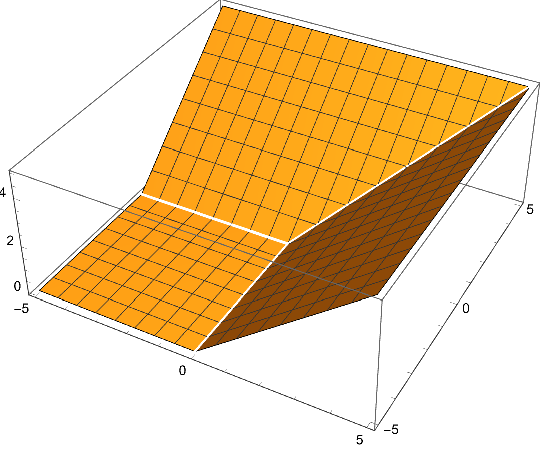
\includegraphics[width=0.3\textwidth]{figs/fig2.1-LinearTropicalPolynomial.pdf}}\quad
        \subcaptionbox{Projection onto $xy$-plane\label{fig:2.2-ProjectionLinearTropicalPolynomial}}{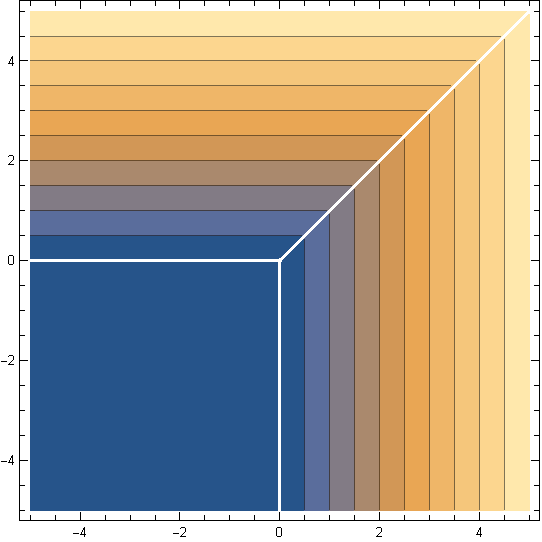
\includegraphics[width=0.25\textwidth]{figs/fig2.2-LinearTropicalPolynomialProjected.pdf}}\quad
        \subcaptionbox{Corner locus\label{fig:2.3-CornerLocus}}{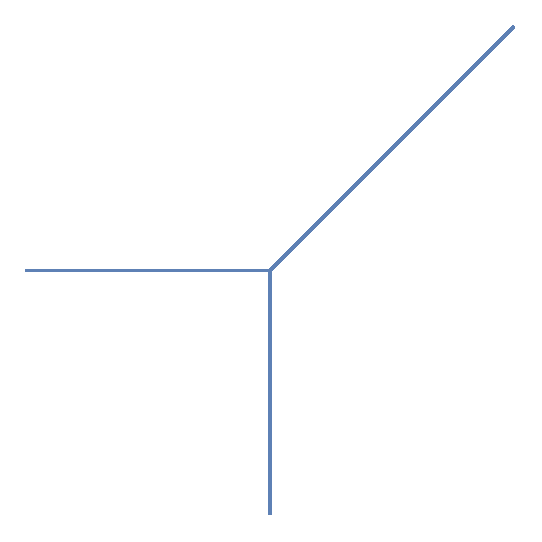
\includegraphics[width=0.25\textwidth]{figs/fig2.3-CornerLocus.pdf}}
        %\caption{This is the caption.}
        \label{fig:2.1-and-2.2-and-2.3}
    \end{figure}
    %https://mathematica.stackexchange.com/questions/169777/listplot3d-with-contours-projected-onto-the-xy-plane
    Observe that the surface is not smooth where the planes meet, this is what we will call the \emph{corner locus} or \emph{tropical hypersurface}.
    %In two variables we have a PICTURE. The polynomial $x\oplus y\oplus 0$ is actually $\max(x,y,0)$. This picture is actually the projection of the corner locus. In 3D we can visualize this better.
\end{Ex}

\begin{Def}
    The \term{tropical hypersurface} $V(\Trop(p))$ is the codimension 1 locus in $\bR^n$ where the function is non-linear (corner locus).
\end{Def}

\begin{Ex}
If we consider higher degree tropical polynomials, they will become linear in the usual sense. Consider 
$$p(x)=3x^2=3\odot x\odot x=3+x+x=3+2x$$
which is indeed linear.
\end{Ex}

\subsection{Valued fields}

\begin{Def}
The field of \term{Puiseux series} or rational functions over $\bC$ is $\bC(t)$ where the elements are of the form 
$$f(t)=\sum_{i=k_0}^\infty a_it^{i/n}.$$
The lower bound $k_0$ could be negative and the exponents, are rational with bounded denominators. 
\end{Def}

Consider the valuation 
$$\val_0\:\bC(t)\to\bR\cup\set{\infty},\begin{cases}
    0\mapsto \infty\\
    f\mapsto\text{order of vanishing at }0.
\end{cases}$$
This order of vanishing is the value $\al$ such that $f/t^\al$ approaches a finite non-zero value. The corresponding coefficient in the series expansion of $f$ for this value is called the valuation coefficient.

\begin{Ex}
    What happens to the order of vanishing when you add two functions? Consider $f=t^2,\ g=t^3$, then $f+g=t^2+t^3$ which has order of vanishing $2$. Observe that $2=\min(2,3)$.
\end{Ex}
In general what happens is that
$$\val_0(f_1+f_2)\geq\min(\val_0 f_1,\val_0 f_2),\word{and}\val_0(f_1f_2)=\val_0(f_1)+\val_0(f_2).$$

We can do algebraic geometry over this field! Let $K$ be the field of rational functions, if $p(\un x)\in K\bonj{\un x}$ then we consider the algebraic variety
$$X=V(p)=\set{\vec{x}\:p(\vec{x})=0}\subseteq K^n.$$
Taking the image through the $n$-fold valuation, we will obtain a set in $\left(\bR\cup\set{\infty}\right)^n$. The tropicalization of $X$ is the image via this map:
\begin{figure}[h!]
    
\centering
\tikzset{every picture/.style={line width=0.75pt}} %set default line width to 0.75pt        

\begin{tikzpicture}[x=0.75pt,y=0.75pt,yscale=-1,xscale=1]
%uncomment if require: \path (0,300); %set diagram left start at 0, and has height of 300

%Straight Lines [id:da2454102694181276] 
\draw    (235,63) -- (299,63) ;
\draw [shift={(301,63)}, rotate = 180] [color={rgb, 255:red, 0; green, 0; blue, 0 }  ][line width=0.75]    (10.93,-3.29) .. controls (6.95,-1.4) and (3.31,-0.3) .. (0,0) .. controls (3.31,0.3) and (6.95,1.4) .. (10.93,3.29)   ;
%Straight Lines [id:da5779705315012776] 
\draw    (241,113) -- (298,113) ;
\draw [shift={(300,113)}, rotate = 180] [color={rgb, 255:red, 0; green, 0; blue, 0 }  ][line width=0.75]    (10.93,-3.29) .. controls (6.95,-1.4) and (3.31,-0.3) .. (0,0) .. controls (3.31,0.3) and (6.95,1.4) .. (10.93,3.29)   ;
\draw [shift={(241,113)}, rotate = 180] [color={rgb, 255:red, 0; green, 0; blue, 0 }  ][line width=0.75]    (0,5.59) -- (0,-5.59)   ;

% Text Node
\draw (208,53.4) node [anchor=north west][inner sep=0.75pt]    {$K^{n}$};
% Text Node
\draw (303,53.4) node [anchor=north west][inner sep=0.75pt]    {$(\bR\cup\set{\infty})^{n}$};
% Text Node
\draw (202,103.4) node [anchor=north west][inner sep=0.75pt]    {$V( p)$};
% Text Node
\draw (304,99.4) node [anchor=north west][inner sep=0.75pt]    {$\overline{\operatorname{val}_0( V( p))}$};
% Text Node
\draw (172,153.4) node [anchor=north west][inner sep=0.75pt]    {$\{\vec{x} :p(\vec{x}) =0\}$};
% Text Node
\draw (302,153.4) node [anchor=north west][inner sep=0.75pt]    {$\operatorname{Trop}( V( p))$};
% Text Node
\draw (210.4,98) node [anchor=north west][inner sep=0.75pt]  [rotate=-270]  {$\subseteq $};
% Text Node
\draw (328.4,98) node [anchor=north west][inner sep=0.75pt]  [rotate=-270]  {$\subseteq $};
% Text Node
\draw (229.6,127) node [anchor=north west][inner sep=0.75pt]  [rotate=-90]  {$=$};
% Text Node
\draw (346.6,127) node [anchor=north west][inner sep=0.75pt]  [rotate=-90]  {$=$};
% Text Node
\draw (172,53.4) node [anchor=north west][inner sep=0.75pt]    {$\operatorname{val}_0\:$};


\end{tikzpicture}

\end{figure}\\
and here $\Trop(V(p))$ is the tropical hypersurface for $p$.
\begin{Ex}
    Consider the polynomial in $K\bonj{x,y}$ 
    $$p(x,y)=tx+y+t^2,$$
    then the variety is $X=\set{(x,y)\: tx+y+t^2=0}$ which we can solve to $y=-tx-t^2$.\par 
    If we choose $x=0$ then $y$ becomes $-t^2$. Now we take the valuation of $(0,-t^2)$ and so $(\infty,2)\in\Trop(X)$.
\end{Ex}

\subsection{Amoebas}

Let us return to the usual stage and consider $p\in\bC[\un x]$ which defines an algebraic variety $X=V(p)\subseteq\bC^n$. Now consider the map which sends every coordinate's modulus to its logarithm in base $t$: 
$$\bC^n\to\left(\bR\cup\set{-\infty}\right)^n,\quad (z_1,\dots,z_n)\to(\log_t|z_1|,\dots,\log_t|z_n|).$$


The image of $X$ under this map, $\log_t(X)$, is the $t$-amoeba of $X$. If we take the limit as $t\to\infty$ then we get the \emph{spine} of the amoeba. 

\begin{Ex}
    When $p(x,y)=x+y-1$ then we can describe $V(p)$ via the parametrization $(x,1-x)$. So the corresponding $t$-amoeba in the real case is 
    $$\set{(\log_t|x|,\log_t|1-x|)\: x\in\bR}$$
    and we ordinarily take the limit, we see that the functions converge to zero point-by-point. But the set is actually approaching the spine!
    \begin{figure}[h!]
        \centering
        \subcaptionbox{$X=V(x+y-1)$\label{fig:2.4-Variety}}{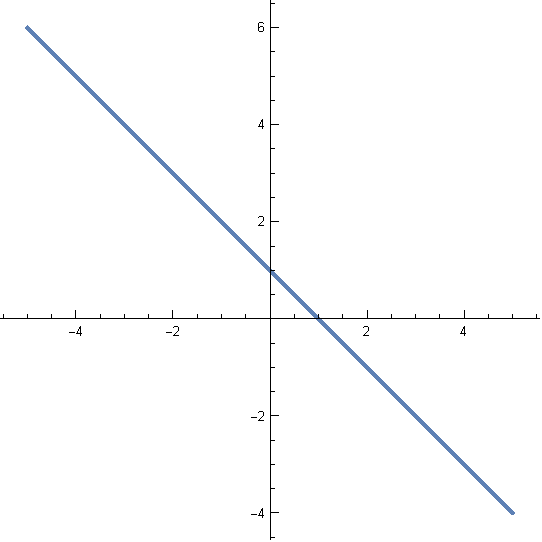
\includegraphics[width=0.25\textwidth]{figs/fig2.4-V(x+y-1).pdf}}\quad
        \subcaptionbox{$2$-amoeba of $X$\label{fig:2.5-2Amoeba}}{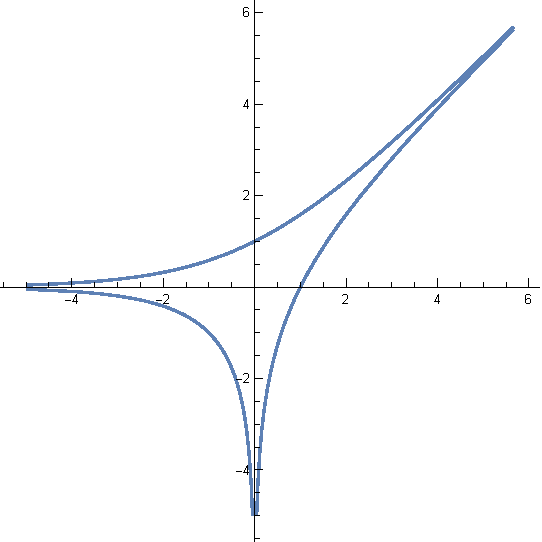
\includegraphics[width=0.25\textwidth]{figs/fig2.5-2amoeba.pdf}}\quad
        \subcaptionbox{Sequence of amoebas as $t\to\infty$\label{fig:2.6-ApproxAmoebas}}{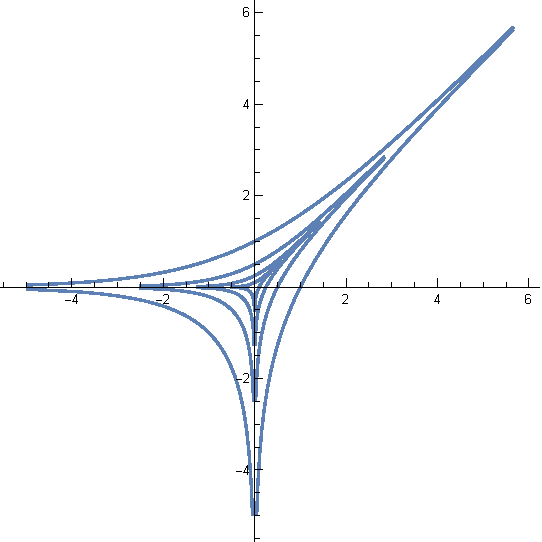
\includegraphics[width=0.25\textwidth]{figs/fig2.6-ApproximatingAmoebas.pdf}}
        %\caption{This is the caption.}
        \label{fig:2.4-thru-2.6}
    \end{figure}
\end{Ex}

Observe that the spine approaches the tropical hypersurface associated to $p$. In other words we have that the tropical hypersurface is $\lim_{t\to\infty}\log_t(V(p))$.

\subsection{Degenerations}
We may parametrize any algebraic variety with a time variable, then converting the information to a graph, edges code the information about how fast the node forms related to the length.\par
Consider a family of \red{of what, what is this family of?! Stuff? Curve in P1xP1 which eventually becomes P2?}
\begin{figure}[h!]
    \centering
    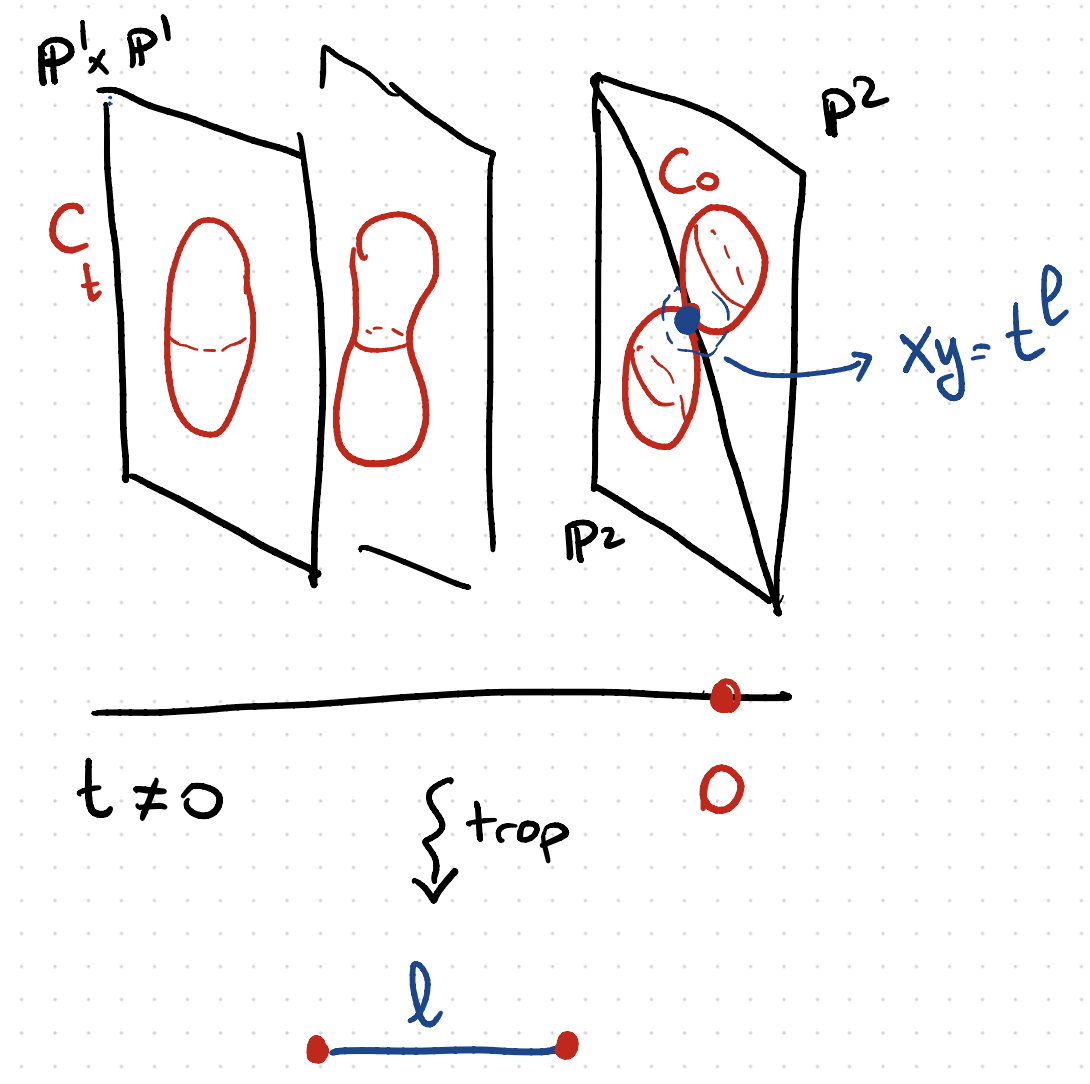
\includegraphics[width=0.5\textwidth]{figs/fig1.1.png}
\end{figure}

It is too early to understand this point of view. We will set everything up to get to it.\par 
In general, the big idea will be to explore and understand these perspectives in the case of plane curves. We want to show how they are equivalent and then recover classical algebraic geometry results in terms of tropical geometry.

\section{Day 3|20230825}

Recall that the last time we discussed the classical (25 to 30 years old) ways to get to tropical geoemtry. We now would like to answer the question
\begin{significant}
    Where do tropical numbers come from?
\end{significant}
So let us begin with an applications problem and see how the tropical numbers arise from the context of the problem.

\subsection{Tropical Arithmetics}%%%Based on TropicalNumbers.pdf

\subsubsection{Minimizing Tolls}

Consider a set of cities connected by a network of toll-ways:
\begin{figure}[h!]
    \centering
    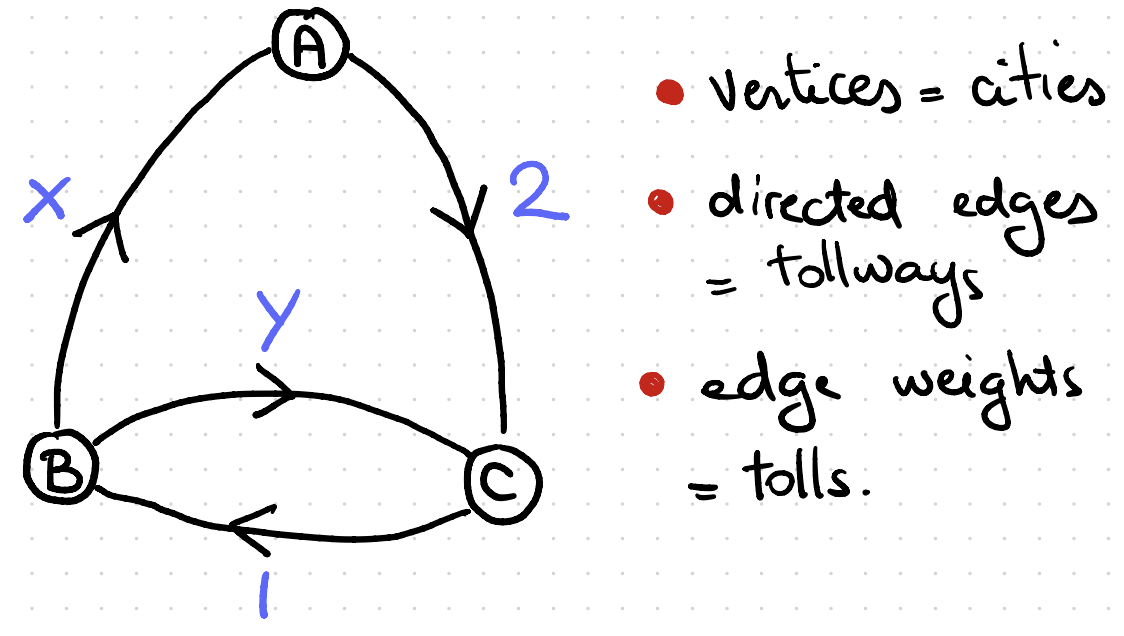
\includegraphics[width=0.5\textwidth]{figs/fig1.2.png}
\end{figure}
If we only care about minimizing toll expenses when traveling, what would be the cheapest way to go from one given city to another? Let us record the information as an incidence matrix:
$$M_{ij}=\text{price of going from city }i\text{ to city }j\text{ in at most one trip}\To M=\threebythree{0}{\infty}{2}{x}{0}{y}{\infty}{1}{0}$$
In this matrix, the rows determine the outbound city, while the columns are the destination. Each entry records the cost of a toll and tolls are considered to be infinite when the road does not exist. We can also think of $M$ as recording the cheapest toll to go from one city to another with at most one move.\par 
How would we compute the best strategy of going from city $i$ to $j$ in \emph{at most two trips}? If for example we want to find trips from $A$ to $B$ in two steps then we have three choices:
$$AAB,\quad ABB,\quad ACB.$$
The costs of each one are 
$$(0,\infty),\quad (\infty,0),\quad (2,1)$$
so we sum them and take the minimum. That will be the optimal route from $A$ to $B$ in two steps. In fact, if we relate this to the entries of the matrix $M$, we could use $M^2$. However we must redefine our basic operations as follows: 
$$+=\min,\quad\.=+$$
So we have the identification 
$$(1,2)\text{ entry of }M^2=\sum_{j=1}^{3}M_{1k}M_{k2}=\min(M_{11}+M_{12},M_{12}+M_{22},M_{13}+M_{32}).$$
In general:
\begin{align*}
    \threebythree{0}{\infty}{2}{x}{0}{y}{\infty}{1}{0}^2&=\threebythree{\min\threebyone{0+0}{\infty+x}{2+\infty}}{\min\threebyone{0+\infty}{\infty+0}{2+1}}{\min\threebyone{0+2}{\infty+y}{2+0}}{\min\threebyone{x+0}{0+x}{y+\infty}}{\min\threebyone{x+\infty}{0+0}{y+1}}{\min\threebyone{x+2}{0+y}{y+0}}{\min\threebyone{\infty+0}{1+x}{0+\infty}}{\min\threebyone{\infty+\infty}{1+0}{0+1}}{\min\threebyone{\infty+2}{1+y}{0+0}}\\
    &=\threebythree{0}{3}{2}{x}{\min(0,y+1)}{\min(x+2,y)}{1+x}{1}{\min(0,1+y)}.
\end{align*}
Observe that $1+y$ can be the minimum in the diagonal when we allow \emph{negative tolls}.
\begin{Rmk}
If we disallow negative tolls, the products $M^n$ eventually stabilize to a matrix whose entries record the cheapest way to get from one city to another in $n$ steps.
\end{Rmk}
This gives us an intuition that minimization problems correspond to linear algebra problems over $(\bT,+,\.)$ which is precisely $(\bR\cup\set{\infty},\min,+)$.

\subsubsection{Forgetting phases}

Recall that any complex number can be written as $z=re^{i\te}$ where $r\geq 0$. Consider the map $T_t\:\bC\to\set{-\infty}\cup\bR,\quad z\mapsto\log_t(r)$.
\begin{figure}[h!]
    \centering
    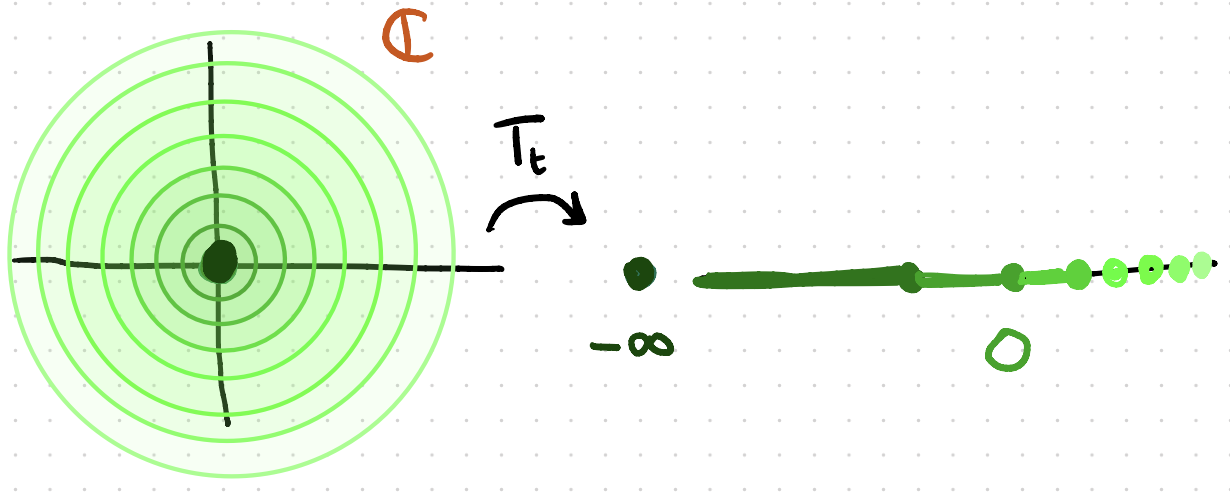
\includegraphics[width=0.5\textwidth]{figs/fig1.3.png}
\end{figure}
This map is surjective, and this we can see by checking it is right-invertible. Observe that:
$$
\left\lbrace
\begin{aligned}
    &T_t^{-1}(x)=\set{t^xe^{i\te}}\subseteq\bC,\word{for}x\in\bR,\\
    &T_t^{-1}(-\infty)=0.
\end{aligned}
\right.
$$
With this in hand, we wish to define an exotic addition and multiplication on $\set{-\infty}\cup\bR$ using $T_t$. We will dequantize!\par 
We begin with \textbf{hyper-addition}, the output will be a subset of $\set{-\infty}$ so it's not a binary operation by itself. 
$$x\diamondplus_t y\:= T_t(T_t^{-1}(x)+T_t^{-1}(y))=\bonj{\log_t(|t^x-t^y|),\log_t(t^x+t^y)}.$$
This is an interval in $\set{-\infty}\cup\bR$, in order to make $\diamondplus_t$ into an operation we take a limit:
\begin{figure}[h!] 
    \centering
\begin{tikzpicture}[x=0.75pt,y=0.75pt,yscale=-1,xscale=1]
%uncomment if require: \path (0,300); %set diagram left start at 0, and has height of 300

%Straight Lines [id:da5156276968518897] 
\draw    (85,62.6) -- (142,62.99) ;
\draw [shift={(144,63)}, rotate = 180.39] [color={rgb, 255:red, 0; green, 0; blue, 0 }  ][line width=0.75]    (10.93,-3.29) .. controls (6.95,-1.4) and (3.31,-0.3) .. (0,0) .. controls (3.31,0.3) and (6.95,1.4) .. (10.93,3.29)   ;

%Straight Lines [id:da8224691621679702] 
\draw    (96,133) -- (144,133.38) ;
\draw [shift={(146,133.4)}, rotate = 180.46] [color={rgb, 255:red, 0; green, 0; blue, 0 }  ][line width=0.75]    (10.93,-3.29) .. controls (6.95,-1.4) and (3.31,-0.3) .. (0,0) .. controls (3.31,0.3) and (6.95,1.4) .. (10.93,3.29)   ;
%Straight Lines [id:da27001319663870027] 
\draw    (57,77) -- (57,118) ;
\draw [shift={(57,120)}, rotate = 270] [color={rgb, 255:red, 0; green, 0; blue, 0 }  ][line width=0.75]    (10.93,-3.29) .. controls (6.95,-1.4) and (3.31,-0.3) .. (0,0) .. controls (3.31,0.3) and (6.95,1.4) .. (10.93,3.29)   ;
%Straight Lines [id:da8909494911629017] 
\draw    (195,83) -- (195,120) ;
\draw [shift={(195,122)}, rotate = 270] [color={rgb, 255:red, 0; green, 0; blue, 0 }  ][line width=0.75]    (10.93,-3.29) .. controls (6.95,-1.4) and (3.31,-0.3) .. (0,0) .. controls (3.31,0.3) and (6.95,1.4) .. (10.93,3.29)   ;

% Text Node
\draw (34,53.4) node [anchor=north west][inner sep=0.75pt]    {$x\diamondplus_t y$};
% Text Node
\draw (34,123.4) node [anchor=north west][inner sep=0.75pt]    {$x\ +_{t} \ y$};
% Text Node
\draw (152,53.4) node [anchor=north west][inner sep=0.75pt]    {$x\diamondplus y=\lim _{t\rightarrow \infty } x\diamondplus_t y$};
% Text Node
\draw (152,123.4) node [anchor=north west][inner sep=0.75pt]    {$x+y=\max( x,y)$};
% Text Node
\draw (60,98.5) node [anchor=west] [inner sep=0.75pt]  [font=\scriptsize]  {$\max$};
% Text Node
\draw (114.5,59.4) node [anchor=south] [inner sep=0.75pt]  [font=\scriptsize]  {$\displaystyle\lim _{t\rightarrow \infty }$};
% Text Node
\draw (121,129.8) node [anchor=south] [inner sep=0.75pt]  [font=\scriptsize]  {$\displaystyle\lim _{t\rightarrow \infty }$};
% Text Node
\draw (197,102.5) node [anchor=west] [inner sep=0.75pt]  [font=\scriptsize]  {$\max$};


\end{tikzpicture}

\end{figure}

\begin{Rmk}
Note that $\diamondplus$ is still a hyperoperation. Its output is not a singleton \emph{only} when a dding a number to itself:
$$x\diamondplus y=\begin{cases}
    \max(x,y),\quad x\neq y\\
    \bonj{-\infty,x},\quad x=y
\end{cases}$$
\end{Rmk}

Formally this process, taking a limit of a family of operations, is known as \emph{dequantization}.\par

In the case of multiplication, things go a lot smoother when defining it:

$$x\.y =T_t\bonj{T^{-1}(x)\.T^{-1}(y)}=\log_t\bonj{(t^xe^{i\te})(t^ye^{i\vf})}=\log_t\left(t^{x+y}e^{i(\te+\vf)}\right)$$

Separating the logarithm we get $(x+y)+\log(e^{i(\te+\vf)})/\log(t)$, then letting $t$ grow without bound we see that the operation converges to $x+y$. 

\begin{Ex}
    Let us consider a small example like summing $2$ and $4$. Observe that 
    $$4\diamondplus_t 2=T_t(T_t^{-1}(4)+T_t^{-1}(2))=T_t\left(t^4e^{i\te}+t^2e^{i\vf}\right)$$
    and the term on the inside can be simplified to $t^{4}(e^{i\te}+t^{-2}e^{i\vf})$. $T_t$ takes that expression to
    $$4+\log_t(e^{i\te}+t^{-2}e^{i\vf})=4+\frac{\log(e^{i\te}+t^{-2}e^{i\vf})}{\log t}.$$
    What happens if we take the limit as $t\to\infty$? We get an independent from $t$ result! 
    The term on the right vanishes and we are left with $4=\max(4,2)$. So it got a tad bit better, but it's still a hyperoperation!
\end{Ex}

\begin{Ej}
Check how the definition of $+$ and $\.$ extend to the \emph{number} $-\infty$.
\end{Ej}

\begin{ptcb}
The point of this exercise is to operate $-\infty$ with finite numbers and itself.\par
For a finite $x$ we will find $x+(-\infty)$. This is the limit of the previous hyperoperation:
$$x\diamondplus_t(-\infty)=T_t(T_t^{-1}(x)+T_t^{-1}(-\infty))=T_t(T_t^{-1}(x)+0)=T_t(T_t^{-1}(x))=x.$$
If we let $t$ grow, the result doesn't change and so this goes according to $\max(x,-\infty)=x$.\par 
On the other hand when taking the product:
$$x\.(-\infty)=T_t\bonj{T^{-1}(x)\.T^{-1}(-\infty)}=T_t\bonj{T^{-1}(x)\.0}=T_t(0)=\log_t(0)\to-\infty$$
which is also similar to the notion of $x+(-\infty)=-\infty$.\par 
We can now proceed to operate $-\infty$ with itself:
$$(-\infty)\diamondplus_t(-\infty)=T_t(0)=\log_t(0)=-\infty=\max(-\infty,-\infty),$$
and when taking the product:
$$(-\infty)\.(-\infty)=T_t(0)\log_t(0)=-\infty=(-\infty)+(-\infty)$$
where the last sum is a sum in the usual sense.
\end{ptcb}

So, summarizing this process:
\begin{itemize}
    \item We forgot about the phase of the complex numbers and only looked at them radially. 
    \item The modulus of these numbers was scaled logarithmically.
    \item Finally we took the limit of these operations and obtained the desired (somewhat) result.
\end{itemize}
This is known as Maslov\footnote{Viktor Pavlovich Maslov (1930615-20230803)} dequantization and with this we can see $(\bT,+,\.)$ as $(\set{-\infty}\cup\bR,\max,+)$. Also, we will abbreviate $\lim_{t\to\infty}T_t$ with $T_{t\to\infty}$

\section{Interim}
%%valued fields

\section{Day 4|20230828}

We have seen where our ideas come from. Certain kinds of minimization problems give rise to our tropical numbers. Also by expressing complex numbers in a logarithmic scale without phase then when inducing a sum we actually get a hypersum. The way we converted into an operation is by taking a limit. Then the algebraic structure we obtained was once again the tropical numbers. Let us talk about the perspective of valued fields.
\subsubsection{Puiseux series}
Recall from our times in Calculus 1 that when resolving indeterminate limits, the relevant information is contained in the order of vanishing of the function.

\begin{Ex}
    Consider the limit $\lim_{t\to 0}\frac{\sin(x)}{x}=1$. Near $t=0$ we have 
    $$\sin(t)=t+o(t)\sim t^1\word{and}\frac{1}{t}=t^{-1}\word{so}t^1t^{-1}=t^0=1.$$
\end{Ex}

From this, we care to study the orders of zeroes and poles of Laurent series. In order to extend the class of functions to an algebraically closed field, we consider Puiseux series, or rational functions. We can identify Puiseux series as 
$$\bC\set{\set{t}}=\bigcup_{n\in\bN}\bC(t^{1/n}).$$
Concretely, elements here are Laurent series with rational exponents and the exponents of terms with non-zero coefficients have a common denominator. 
\begin{Ex}
    The series $\sum_{k=-37}^{\infty}t^{k/42}$ is a Puiseux series while $\sum_{k=1}^\infty t^{1/k}$ is not because the exponents keep getting smaller and smaller.
\end{Ex}
This is the most natural algebraically closed field with a \emph{canonical} valuation. This is the function:
$$\val: \bC\set{\set{t}}\to\bR\cup\set{\infty},\begin{cases}
    0\mapsto\infty\\
    t^{p/q}+\text{higher order}\mapsto p/q
\end{cases}$$

In other words the valuation sends $\sum_{k=k_0}^\infty a_kt^{q_k}$ to $q_{k_0}$.
\begin{Prop}
The previous valuation enjoys the following properties:
\begin{enumerate}[i)]
    \item $\val(\al\.\bt)=\val(\al)+\val(\bt)$.
    \item $\val(\al+\bt)\geq\min(\val(\al),\val(\bt))$.
\end{enumerate}
Equality holds when $\val(\al)\neq\val(\bt)$.
\end{Prop}
So if we decide to define operations on $\bR\cup\set{\infty}$ by inducing them from the operations on $\bC\set{\set{t}}$, then we obtain
\begin{align*}
    &x\diamondplus y=\val\left(\val^{-1}(x)+\val^{-1}(y)\right),
    &x\. y=\val\left(\val^{-1}(x)\.\val^{-1}(y)\right).
\end{align*}
Now $\.$ coincides with usual addition and $+$ is the hyperoperation
$$x\diamondplus y=\begin{cases}
    \min(x,y)\word{when}x\neq y,\\
    [\min(x,y),\infty]\word{when}x=y.
\end{cases}$$
\begin{Ex}
    If we try to sum $0$ with itself, we get 
    $$0\diamondplus 0=\val\left((a_0+a_1t^{q_1}+\dots)+(-a_0+b_1t^{r_1}+\dots)\right)$$
\end{Ex}
The only natural way to turn this into an operation is to define $x+y=\min(x,y)$. In conclusion, the field of Puiseux series with the order of vanishing and poles is congruent to $(\bT,+,\.)$ which in this case is $\left(\bR\cup\set{\infty},\min,+\right)$.

\subsection{The Tropical Semifield}

\begin{Def}
    The \term{tropical semifield} is $(\bT,+,\.)$ where we can choose:
    \begin{itemize}
        \item $\bT=\bR\cup\infty$, $+=\min$ and $\.=+$, the min convention.
        \item $\bT=\set{-\infty}\cup\bR$, $+=\max$ and $\.=+$, the max convention.
    \end{itemize}
\end{Def}

There is a natural isomorphism between the two choices given by $x\mapsto -x$. As we have mentioned, different contexts may be more natural than the other when using certain conventions. We will tipically use the $\max$ convention. 

\begin{Prop}
The following algebraic properties hold for $(\bT,+,\.)$:
\begin{enumerate}[i)]
    \item $0_\bT=-\infty$.
    \item $1_{\bT}=0$.
    \item $x+y=0_\bT$ only has the solution $x=y=0_\bT$. This means that only $-\infty$ has an additive inverse.
    \item Addition is idempotent: $x+x=x$.
    \item Every non-zero element has a multiplicative inverse: $1/x=-x$.
\end{enumerate}
\end{Prop}

\begin{ptcbp}
    \begin{enumerate}[i)]
    \item Observe that $x+0_\bT=\max(x,-\infty)=x$.
    \item $x\.1_\bT=x+0=x$.
    \item $x+y=0_\bT\iff \max(x,y)=-\infty\To x=y=-\infty$.
    \item $x+x=\max(x,x)=x$.
    \item $x\.(1/x)=x+(-x)=0=1_\bT$.
\end{enumerate}
\end{ptcbp}
Observe that it is not possible to adjoin formal additive inverses. Suppose that for $x\in\bT$ there exists a $y$ such that $x+y=0_\bT$, then 
$$(x+x)+y=x+y=0_\bT\word{and}x+(x+y)=x+0_\bT=x\word{but}x\neq 0\_\bT.$$
This means that any invertible element necessarily has to be $-\infty$.

\begin{Ej}[2-]
Which other algebraic properties do these operations enjoy? We have claimed for example that $+$ is associative. Prove this.\par 
Are the operations commutative? Do they distribute with respect to each other?
\end{Ej}

\begin{Prop}[Weird Fun Facts]
Recall that the usual Pascal Triangle is built by adding the \emph{previous two} elements to get the next one. In the tropical case we have 
$$
%https://tex.stackexchange.com/questions/17522/pascals-triangle-in-tikz
\begin{tikzpicture}
    \foreach \n in {0,...,2} {
      \foreach \k in {0,...,\n} {
        \node at (\k-\n/2,-\n) {$1_\bT$};
      }
    }
    \end{tikzpicture}
    \word{\raisebox{2.5em}{=}}%tex.se/47016
    \begin{tikzpicture}
        \foreach \n in {0,...,2} {
          \foreach \k in {0,...,\n} {
            \node at (\k-\n/2,-\n) {$0$};
          }
        }
        \end{tikzpicture}
    $$
    and this extends downwards with the same pattern.\par 
    In the case of the tropical binomial theorem, the identity is
    $$(x+y)^n=x^n+y^n\iff n\max(x,y)=\max(nx,ny).$$
\end{Prop}

\begin{Ej}[2]
Recall that the coefficients in the expansion for the binomial theorem are the corresponding elements in the rows of the Pascal Triangle. Verify if the coefficients agree in the tropical case for the binomial theorem.
\end{Ej}


\subsubsection{The Optimal Assignment Problem}

Suppose we have $n$ jobs for $n$ workers. Each worker can only work one job and once the job is taken, no one else can do it. We wish to assign a job to each worker in order to maximize our company's profit.

\begin{Ex}
    As a little example consider Alice and Bob's hydroponics farm. When working with the weeds Alice produces $5$ credits while working with the water she produces $6$. On the other hand Bob produces $3$ and $5$ respectively.\par 
    It is easy to see that Alice should be assigned to to the weed and Bob to the water in order to maximize. But let us apply what we know with tropical arithmetics.\par 
    Call 
    $$M_{ij}=\text{amount of credits work }i\text{ produces when doing job }j.$$
    Then we can summarize the previous information in a matrix 
    $$M=\twobytwo{5}{6}{3}{5}$$
    and if we take the tropical determinant (which is really a permanent since we lack subtraction) we get
    $$\Trop\det M=5\.5+6\.3=\max(5+5,6+3)=10$$
    which is the maximal profit we can make by assigning our workers.
\end{Ex}

\begin{Ej}
    Do the following:
    \begin{itemize}
        \item[(1-)] Construct a $3\x3$ matrix with non-permuted entries such that there's more than one possible assignment for the optimal jobs.
        \item[(1)] Use the combinatorial definition of permanent to show that the tropical determinant of $M$ is indeed the maximal profit. \hint{The definition of permanent is the same as the determinant but without the $(-1)^{\sgn\sg}$.}
        \item[(5)] Assuming you know the tropical determinant of a matrix, devise a way to identify one job combination which reaches the optimum value. 
    \end{itemize}
\end{Ej}

\section{Day 5|20230830}

The last time we talked about the algebraic structure of the value group of the Puiseux series. We now have plenty of motivation of why would we define the tropical numbers. 

\subsection{Tropical Polynomials and Roots}

An univariate,tropical, (Laurent) monomial is equivalent to an affine linear function with integer coefficients. Such a monomial is an expression of the form 
$$a\odot x^{\odot m},\quad a\in\bT,\quad m\in\bZ.$$

\begin{Ex}
    We have for example:
    $$5x^2\otto 5+2x,\quad 2x^{-3}\otto 2-3x\ (\text{Laurent}).$$
    Also consider $\sqrt 5\odot x^{\odot 3}$ which corresponds to $y=\sqrt{5}+3y$. Notice how the slope is always an integer, meanwhile the translation can be any number.
\end{Ex}

An univariate tropical (Laurent) polynomial is a finite sum of monomials which give rise to a \emph{convex}, continuous, piecewise, affine linear function with integer slopes. 

\begin{Ex}
    Consider the function $-5\odot x^{\odot2}\oplus(-2)\odot x^{\odot-3}\oplus 0$ which corresponds to 
    $$\max(-5+2x,-2-3x,0).$$
    If we graph this functions we obtain
    \begin{figure}[h!]
        \centering
        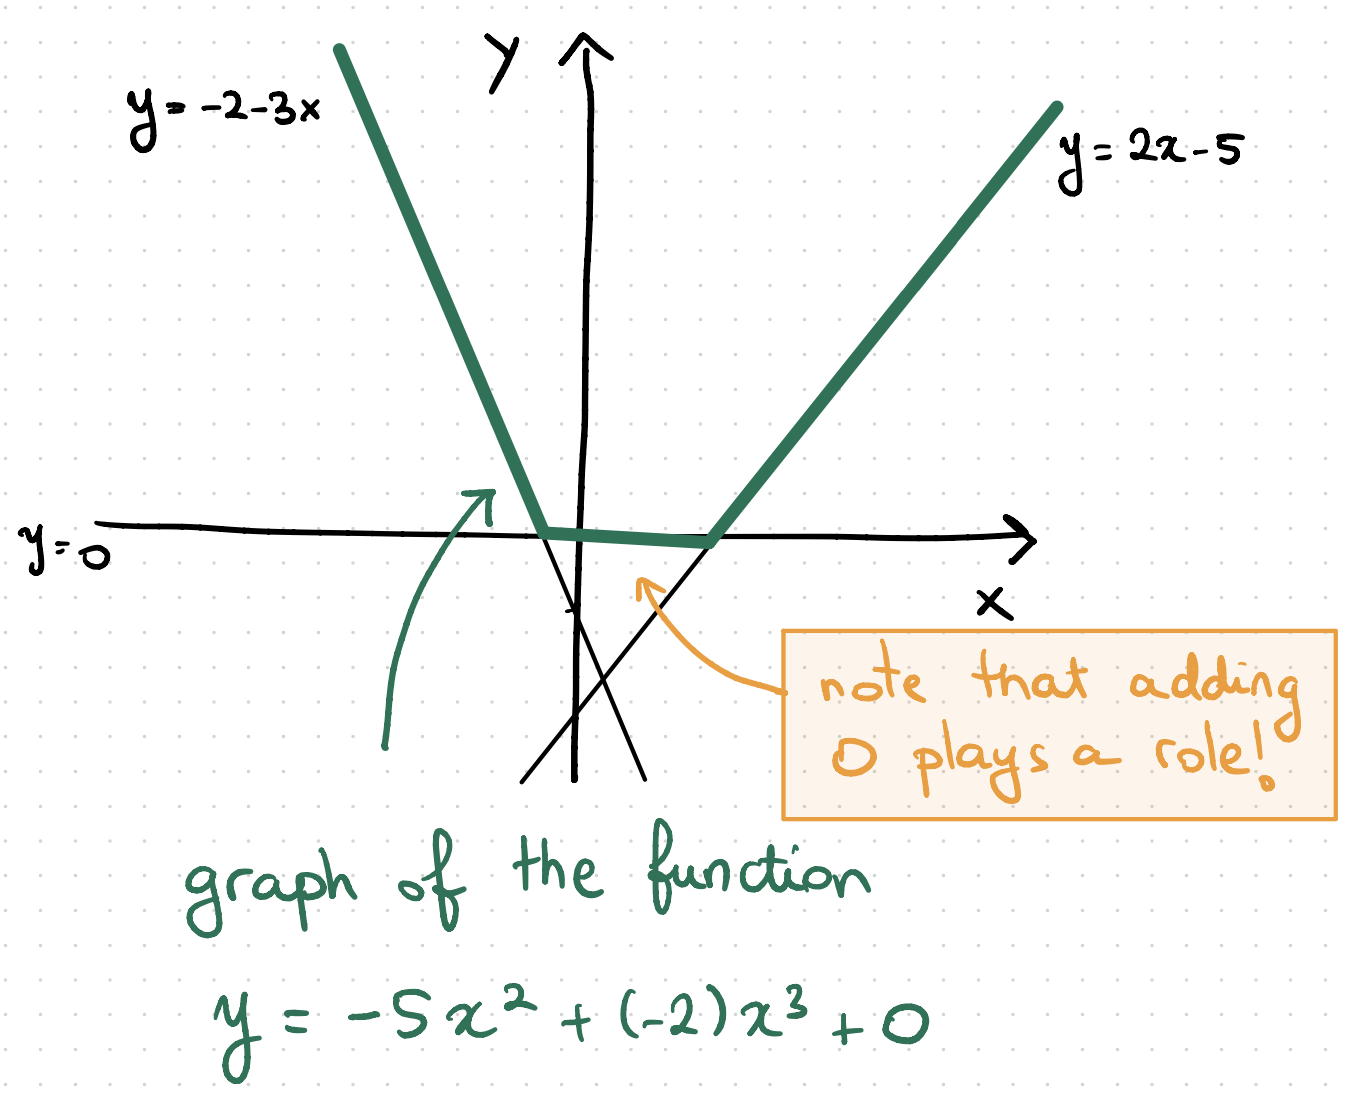
\includegraphics[width=0.5\textwidth]{figs/fig3.1RenzoNotes3.png}
        %\caption{This is the caption.}
        \label{fig:3.1-ConvPLFunc}
    \end{figure}
    Observe that this function is indeed convex, and fulfills all of the previous properties from before. 
\end{Ex}

In fact the map from $\bT[x]$ to convex, affine piecewise linear functions with \emph{finitely} many distinct regions of linearity is surjective. If we don't want to take the finiteness condition into consideration, we have to amplify the domain to tropical Laurent series.\par 
A small measure of care should be taken because there are multiple tropical polynomials which map to the same function.

\begin{Ex}
    Consider the functions 
    $$p_1=x+\frac{1}{x}+0,\quad p_2=x+\frac1x-2.$$
    When converting we get 
    $$\max(x,-x,0),\quad\max(x,-x,-2)$$
    which produce $|x|$ in both cases.
    \begin{figure}[h!]
        \centering
        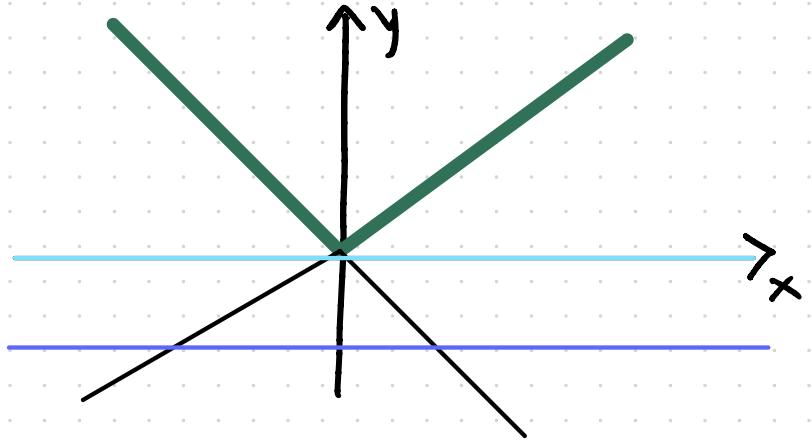
\includegraphics[width=0.5\textwidth]{figs/fig3.2RenzoNotes3.png}
        \caption{Failure of injectivity as both functions map to $|x|$ with $y=0$ and $y=-2$ shown.}
        \label{fig:3.2-InjectivityFailure}
    \end{figure}
    Adding something which is smaller than the minimum value of the function doesn't change it in general. It also doesn't have to be a constant in general. In the previous example, the the monomial $(-4)\odot x^{\odot 1}$ is smaller than any of the linear functions, so adding it changes nothing.
\end{Ex}

To talk about the roots, we will start with a purely combinatorial definition. 

\begin{Def}
    Given a polynomial $p\in\bT[x]$ of degree $d$ we say the following:
    \begin{itemize}
        \item $-\infty$ is a root of $p$ if the slope of the piecewise linear function is non-zero for $x\ll 0$.
        \item $x_0\in\bR$ is a root of $p$ if $p'(x_0)$ is undefined. Observe that the derivative is undefined only when there's a change in slope.
    \end{itemize}
    We say that the \term{multiplicity} of $x_0$ is the difference between slopes across $x_0$. If $-\infty$ is a root, then its multiplicity is equal to the slope of the associated function for $x\ll 0$.
\end{Def}

\begin{Ex}
    Consider the polynomial $x^{\odot2}\oplus1\odot x^1\oplus 0=\max(2x,x,0)$.
    \begin{figure}[h!]
        \centering
        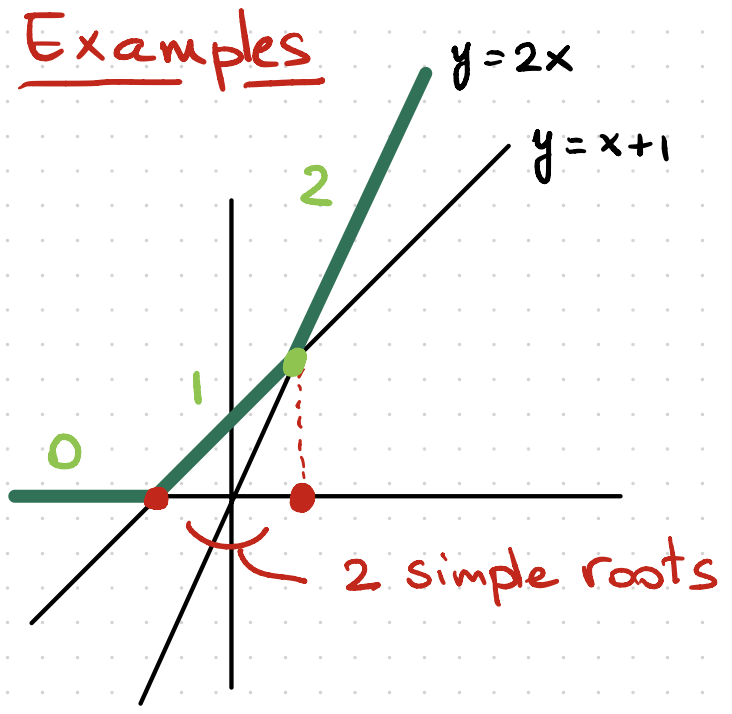
\includegraphics[width=0.5\textwidth]{figs/fig3.3SimpleFiniteRootsTropicalPolynomial.png}
        %\caption{}
        \label{fig:3.3-SimpleFiniteRoots}
    \end{figure}
    We can see that there are changes in slope at $x_1=-1$ and $x_2=1$. The number of roots coincides with the degree of the polynomial as in the usual sense.
\end{Ex}

\begin{Ex}
    Let's remove the zero, recall zero isn't the additive identity, so the polynomial we have is $x^{\odot2}\oplus1\odot x^1=\max(2x,x)$.
    \begin{figure}[h!]
        \centering
        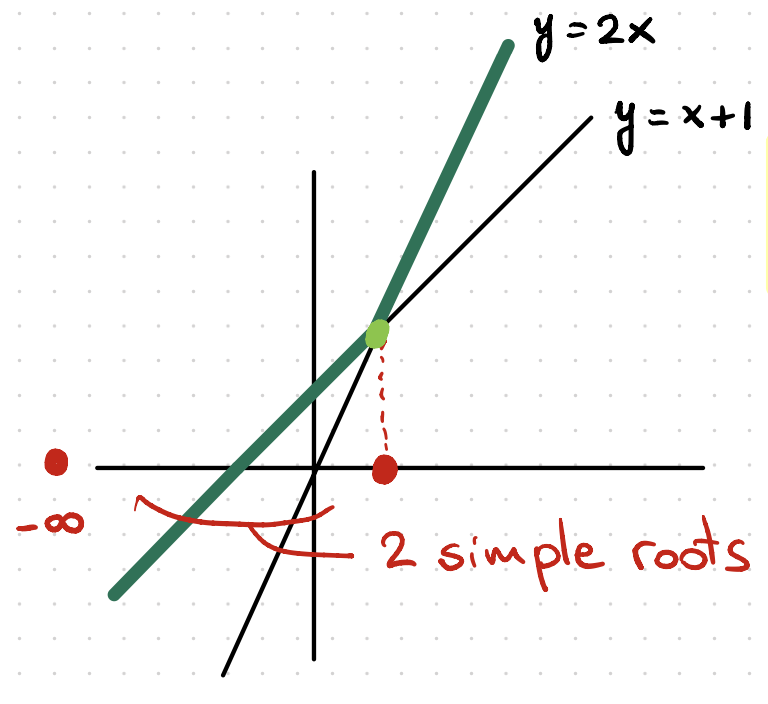
\includegraphics[width=0.5\textwidth]{figs/fig3.4SimpleRootsTropicalPolynomial.png}
        %\caption{}
        \label{fig:3.4-OneFiniteRootOneInfiniteRoot}
    \end{figure}
    Now one of the roots is still $x=1$, but remember that if the slope is non-zero when $x\ll 0$, then $-\infty$ is a root of $p$. This is the case here because the slope is $1$ as $x\to-\infty$. Once again there's two roots $x_1=-\infty$ and $x_2=1$.
\end{Ex}

\begin{Ex}
    Let us change a sign in a coefficient, take $x^2-1\.x^1+0$. But what is tropical subtraction? It's not that, let's convert this slowly into what it's supposed to be:
    $$x^2-1\.x^1+0=(x\.x)+(-1)\.x+0=(2x)+(x+(-1))+0=\max(2x.x-1,0).$$
    \begin{figure}[h!]
        \centering
        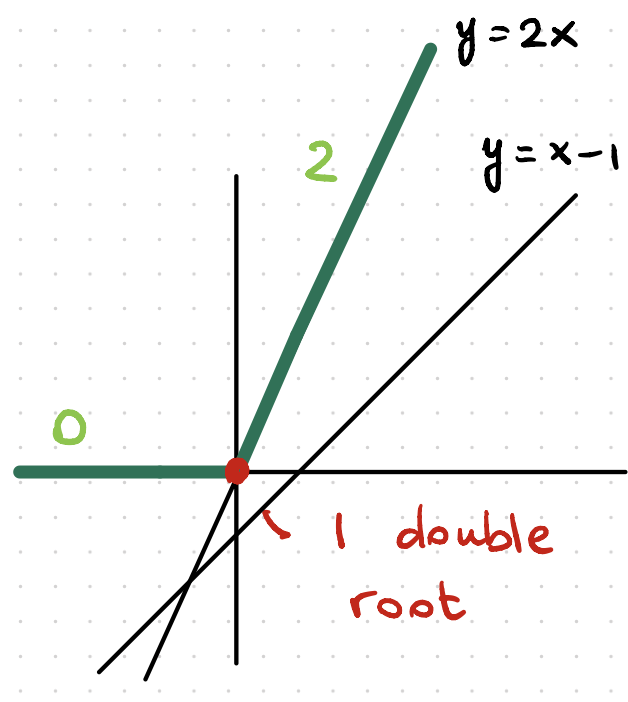
\includegraphics[width=0.5\textwidth]{figs/fig3.5DoubleRootTropicalPolynomial1.png}
        %\caption{}
        \label{fig:3.5-DoubleRoot1}
    \end{figure}
    Observe that because the line $y=x-1$ is below our graphs, it doesn't interfere with the calculation of zeroes. So the only place where there occurs a change in sign is $x=0$. The slope on the right is $2$ and on the left is $0$ so the multiplicity is $2-0=2$.
\end{Ex}

\begin{Ex}
    In a similar fashion, $x^2+0$ also has a double root at $x=0$.
    \begin{figure}[h!]
        \centering
        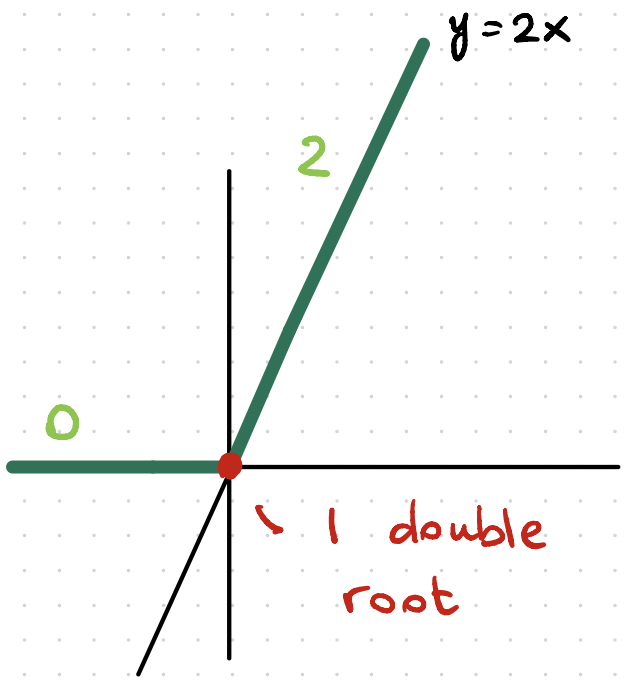
\includegraphics[width=0.5\textwidth]{figs/fig3.6DoubleRootTropicalPolynomial2.png}
        %\caption{}
        \label{fig:3.6-DoubleRoot6}
    \end{figure}
    There is only one change in slope once again at $x=0$ and the difference in slopes is $2$.
\end{Ex}

\begin{Lem}
For a tropical polynomial $p$, a finite $x_0$ is a root of $f$ if and only if when we write the function as a $\max$ of linear functions, at $x_0$ the maximum value is obtained at least twice.\par 
The multiplicity of the root is equal to the difference in the two extremal positions where the $\max$ is attained.
\end{Lem}

This should be more or less obvious. Being a root means that we are an intersection of two lines which are above all the others. It's pretty useful to have this notions around.

Questions arise:
\begin{significant}
    Which functions have only one simple zero at $-\infty$? What would a function with an order 2 zero at $-\infty$ look like?
\end{significant}

\begin{Ej}
    Do the following:
    \begin{itemize}
        \item[(5)] Is it possible for a function to have only a simple zero at $-\infty$? Provide an example of function with one simple zero at $-\infty$ or prove that such function cannot exist. 
        \item[(5)] Do functions with zeroes at $-\infty$ have infinite order at such zero or is it arbitrarily high? If a function has a finite order zero at $-\infty$ provide an example of one with a double zero at $-\infty$. Else, prove that such functions have infinite order at that zero.
    \end{itemize}
\end{Ej}

\section{Day 6|20230901}

How do we know that the notions of roots are natural or useful?

\subsection{Factorization of Tropical Polynomials}

Suppose a polynomial $p\in\bT[x]$ has roots $a_k$ with multiplicity $m_k$. Then we may factor $p$ as a product of linear polynomials 
$$p(x)=c_0\bigodot(x\oplus a_k)^{m_k}.$$
This $p$ is the affine piecewise-linear function, not the formal object. And so, in a sense, $\bT$ is algebraically closed. But instead of proving this, we will sketch the proof to get an idea of how things \emph{work} with a couple of examples.\par 
The idea of the proof is that we check that product does define a P.L. function with the right slopes and then $c_0$ gives the translation factor.
\begin{Ex}
First lets deal with the case where $-\infty$ is not a root. Consider the polynomial 
$$p(x)=(-1)\oplus(-1)\odot x\oplus(-4)\odot x^4=\max(-1,x-1,4x-4).$$
Remember, as in the case of real polynomials, the square and cube terms are still there. The coefficient that foes along them is just $-\infty$. We can graph the polynomial in order to see the roots:
\begin{figure}[h!]
    \centering
    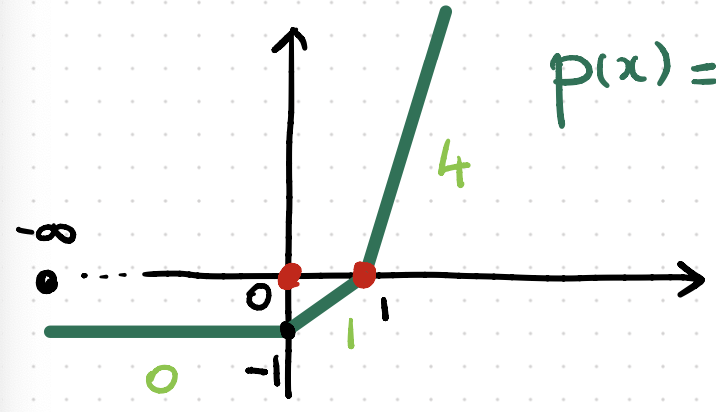
\includegraphics[width=0.5\textwidth]{figs/fig4.1-InfinityNotRoot.png}
    \caption{Graph of $p(x)$ with roots shown}
    \label{fig:4.1-InfinityNotRoot}
\end{figure}
The points where there is a change in slope are $a_1=0$ and $a_2=1$. Then their multiplicities are $1-0=1$ and $4-1=3$ respectively. We may write $p$ as 
$$p(x)=c_0\odot(x\oplus 0)\odot(x\oplus 1)^{3}=c_0+\max(x,0)+\max(3x,3).$$
Whatever function we have, we can write as the sum of three terms. So let us subdivide the tropical line in order to see which terms goes where.
\begin{table*}[h!]
    \centering
    %\arraystretch{1.3}
    \begin{tabular}{rrrr}\toprule
        $x\leq 0$ & $0\leq x\leq 1$ & $1\leq x$\\ \midrule
        $c_0$& $c_0$&$c_0$\\
        $0$&$x$ & $x$\\
        $3$& $3$ & $3x$\\ \midrule
        $c_0+3$&$c_0+3+x$&$c_0+4x$\\
   \bottomrule
    \end{tabular}
    \legend{Behavior of $p(x)$ across $\bT$}
    \end{table*}
    The constant can be determined by plugging in $x=-\infty$. We can see that 
    \begin{align*}
        p(-\infty)&=(-1)\oplus(-1)\odot (-\infty)\oplus(-4)\odot (-\infty)^4=-1\\
        &=c_0\odot(-\infty\oplus 0)\odot(-\infty\oplus 1)^3=c_0\odot0\odot 1^{\odot 3}.
    \end{align*}
    This gives us the equation $c_0+0+3=-1$ which leads us to $c_0=-4$. With this we verify that 
    $$p(x)=\begin{cases}
        -1&x\leq 0\\
        x-1&0\leq x\leq 1\\
        4x-4&1\leq x
    \end{cases}$$
    So in this case $c_0=p(-\infty)-\sum m_ka_k\in\bR$.
\end{Ex}

\begin{Ex}
    We now explore the case where $-\infty$ is a root or a pole. The argument will essentially be the same with a small modification.\par 
    Consider the function $\frac{1}{x}\oplus x$.
    \begin{figure}[h!]
        \centering
        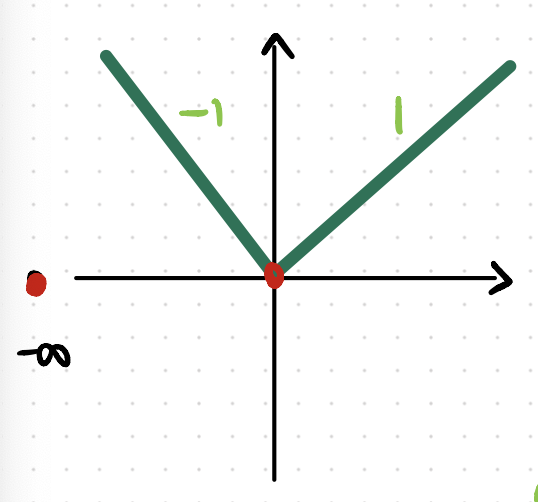
\includegraphics[width=0.5\textwidth]{figs/fig4.2RootAndPoleProof.png}
        %\caption{}
        \label{fig:4.2-RootAndPoleProof}
    \end{figure}
    We have $-\infty$ as a pole of order $1$ and $0$ is a root of order $1-(-1)=2$. So this can be factored as 
    $$p(x)=c_0\odot(x^{-1})\odot(x+\oplus 1)^2$$
    and even if $-\infty$ doesn't give us a particular value for the function, we can still find $c_0=0$ from the equation $p(0)=0$.\par 
    If on the other hand we have a negative slope then we have a zero at $-\infty$. Consider the function $p(x)=x+x^2$:
    \begin{figure}[h!]
        \centering
        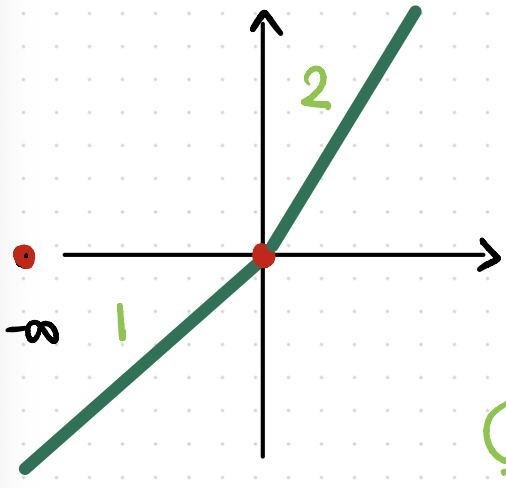
\includegraphics[width=0.5\textwidth]{figs/fig4.3RootsForProof.png}
        %\caption{}
        \label{fig:4.3-RootsForProof}
    \end{figure}
    This function has two simple roots at $-\infty$ and $0$. We may factor it as 
    $$p(x)=c_0\odot(x\oplus-\infty)\odot(x\oplus 0)$$
    and even if $p(-\infty)=-\infty$ we can plug in $0$ to get $0$ back in order to get $c_0=1$.
\end{Ex}

\subsection{Correspondence Theorems}
Recall the maps 
\begin{align*}
    &T_t\: \bC\to\bT\quad(\text{with }\max),\\
    &\val\: \bC\set{\set{t}}\to\bT\quad(\text{with }\min).
\end{align*}
If we consider a polynomial 
$$p(X)\in\bC[X]\word{or}p(x)\in\bC\set{\set{t}}[X]$$
then we can produce a tropical polynomial as follows:
\begin{enumerate}[i)]
    \item Taking the images of the coefficients via $T_t$ or $\val$, and
    \item tropicalizing the operations. 
\end{enumerate}
We hope that if $r\in\bC$ or $r\in\bC\set{\set{t}}$ was a root of $p$, then $\lim_{t\to\infty}T_t(r)$ is a root of the new polynomial.\par
Or the other way around, given $p\in\bT[x]$, we can lift the coefficients to $\bC$ or the Puiseux series via the above maps. We can find the roots of the corresponding polynomials in $\bC[x]$ or $\bC\set{\set{t}}[x]$ and then the image of those roots via $T_t$ or $\val$ are the tropical roots of $p(x)$.

\begin{Ex}
    Consider the polynomial $p(x)=2\odot x\oplus3\in\bT[x]$. We wish to construct a polynomial in $\bC[x]$ which tropicalizes to $p$.Take the polynomial 
    $$q(x)=t^2X+t^3\in\bC[x]$$ 
    where $t>0$ is a parameter. We could certainly add phase as $e^{i\te}$, but that won't change anything. Taking $\log_t$ of the coefficients we get $t^2\mapsto 2$ and $t^3\mapsto 3$. Taking tropical operations we get $2\odot X\oplus 3$ which was our original polynomial.\par 
    If we ordinarily solve $q=0$ we get $X=-t^3/t^2=-t$, which maps to $1$ via $\log_t||$. Lo and behold, this is the same root of $p(x)$. 
\end{Ex}
We can be skeptical because the previous example was linear. So lets amp up the degree a bit.
\begin{Ex}
    Consider the polynomial
    $$q(X)=X^2+t^2X+1\in\bC[X]\xrightarrow[]{\Trop}p(x)=x^2\oplus 2\odot x\oplus 0.$$
    The roots of $p$\red{ADD FIGURE} are located at $-2$ and $2$ but the roots of $q$ are
    $$r_{1,2}=\frac{-t^2}{2}\pm\frac{\sqrt{t^2-4}}{2}.$$
    Even if taking the logarithm seems hard, we are not interested in the logarithm, just the limit! Observe that 
    $$\lim_{t\to\infty}\log_t\left(\frac{-t^2}{2}\left(1+\sqrt{1-\frac{4}{t^2}}\right)\right)=2+0.$$
\end{Ex}
%%%%%%%%%%%% Contents end %%%%%%%%%%%%%%%%

%%%%%%% testing! testing testing testing testing!
\ifx\nextra\undefined
\printindex
\else\fi
\nocite{*}
\bibliographystyle{plain}
\bibliography{bibiTropiGeo.bib}
\end{document} 

